\documentclass[11pt,dvipdfm]{article}
%\documentclass[11pt]{article}
\usepackage{deauthor,times,graphicx,hyperref} 

\usepackage{amsmath, amssymb, amsfonts} %JF: removed amsthm which causes an error due to a duplicate definition

\def\BibTeX{{\rm B\kern-.05em{\sc i\kern-.025em b}\kern-.08em
    T\kern-.1667em\lower.7ex\hbox{E}\kern-.125emX}}


% \newtheorem{definition}{Definition}[section] %depending on the style file used, these lines may need to be commented out
% \newtheorem{theorem}{Theorem}[section]
% \newtheorem{corollary}{Corollary}[section]
% \newtheorem{lemma}{Lemma}[section]

%The following packages are used to make the causal assumptions figure, but are no longer needed since I saved the figure to a separate pdf.
%\usepackage{booktabs}
%\usepackage{tikz}
%\usetikzlibrary{bayesnet}

\usepackage{breakcites} %Fixes citations exceeding the margin!!

% \newtheorem{example}{Example} 
% \newtheorem{theorem}{Theorem}
% \newtheorem{lemma}[theorem]{Lemma} 
% \newtheorem{proposition}[theorem]{Proposition} 
\newtheorem{remark}[theorem]{Remark}
% \newtheorem{corollary}[theorem]{Corollary}
% \newtheorem{definition}[theorem]{Definition}
% \newtheorem{conjecture}[theorem]{Conjecture}
% \newtheorem{axiom}[theorem]{Axiom}
%%%
\newtheorem{dfn}[theorem]{Definition}

%\usepackage{todonotes}
%\newcommand{\jf}[1]{{\bf \color{orange}{jf: #1}}} %JF: commented out these TODO comment macros to make sure I didn't miss removing any.  Put them back if we ever edit this collaboratively again
%\newcommand{\shimei}[1]{{\bf \color{blue}{shimei: #1}}}
\setcounter{topnumber}{2}
\setcounter{bottomnumber}{2}
\setcounter{totalnumber}{4}
\renewcommand{\topfraction}{0.85}
\renewcommand{\bottomfraction}{0.85}
\renewcommand{\textfraction}{0.15}
\renewcommand{\floatpagefraction}{0.7}

% Definitions of handy macros can go here

\newcommand{\dataset}{{\cal D}}
\newcommand{\fracpartial}[2]{\frac{\partial #1}{\partial  #2}}

\begin{document}
\title{Are Parity-Based Notions of AI Fairness Desirable?}
\author{James R. Foulds and Shimei Pan\\ 
University of Maryland, Baltimore County\\ 
\{jfoulds, shimei\}@umbc.edu}


\maketitle
\begin{abstract}
It is now well understood that artificial intelligence and machine learning systems can potentially exhibit discriminatory behavior.  A variety of AI fairness definitions have been proposed which aim to quantify and mitigate bias and fairness issues in these systems.  Many of these AI fairness metrics aim to enforce parity in the behavior of an AI system between different demographic groups, yet parity-based metrics are often criticized for a variety of reasons spanning the philosophical to the practical.  The question remains: are parity-based metrics valid measures of AI fairness which help to ensure desirable behavior, and if so, when should they be used?  We aim to shed light on this question by considering the arguments both for and against parity-based fairness definitions.  Based on the discussion we argue that parity-based fairness metrics are reasonable measures of fairness which are beneficial to maintain in at least some contexts, and we provide a set of guidelines on their use.
\end{abstract}

\section{Introduction}
As artificial intelligence (AI) and machine learning (ML) systems are now widely deployed to automate decisions with substantial impact on human lives and our society including bail and sentencing decisions~\cite{angwin2016machine}, lending~\cite{applecard}, and hiring~\cite{dastin2018amazon}, these systems have come under increasing scrutiny.  According to the 2019 report from the AI Now Institute at New York University, ``\emph{tech companies are,
in fact, deeply aware that algorithmic discrimination is entrenched in the systems with which they are blanketing the world,}'' even if these companies have not always successfully addressed it~\cite{crawford2019ai}. In response to these concerns, a new and rapidly growing field of research on AI fairness has emerged which aims to study these issues and propose solutions.

To date, much of the research on AI fairness ---at least that which has arisen from the computer science community--- has centered around mathematical definitions or metrics which aim to quantify the degree of fairness or bias in an AI/ML system \cite{dwork2012fairness}.  We focus here on fairness in classification algorithms in which an individual's predicted class label is used to make a decision that directly impacts that individual.  For example, a prediction on whether an individual will repay a loan may determine whether that individual is offered a loan.  Thus, if the behavior of the system is unfair or discriminatory it may produce harm to the affected individuals and to the health of our society, due to perpetuating (or even exacerbating) discriminatory patterns in real-world outcomes which are reflected in the training data \cite{barocas2016big}.

Given the predictions made by a classification model, an AI fairness metric produces a score which assesses the extent that the model's behavior is fair or unfair (e.g. if it exhibits harmful behavior such as a bias toward or against a particular demographic group).  With a fairness metric in hand, the typical fair AI approach is to modify machine learning algorithms such that the training procedure penalizes solutions according to their degree of unfairness under the metric, or are constrained to produce a solution where the fairness metric is considered satisfactory \cite{dwork2012fairness}.  Hence, the ``fairness'' of an AI system is improved compared to the same system without this mitigation procedure, to the extent that the chosen metric successfully encodes what it means for the system to be ``fair.''  It is important to note that AI fairness is a complex sociotechnical problem which cannot be solved by the purely technical ``band-aid'' of enforcing a mathematical fairness definition without due consideration of non-technical factors \cite{crawford2019ai}.  Nevertheless, mathematical fairness definitions and learning algorithms that enforce them are valuable tools as part of a solution to unwanted discrimination in AI, which ideally would further consider sociotechnical, contextual, historical, legal, and stakeholder-centric perspectives in the design of the system.  

Many, perhaps even the majority, of proposed AI fairness metrics and fair learning algorithms aim to ensure that different protected demographic groups, e.g. along lines of gender, race, nationality, sexual orientation, age, social class, or political affiliation, are treated similarly overall by the algorithm.  For example, the metrics may enforce that the likelihood of being offered a loan, or being admitted to college, as determined by an AI algorithm, is approximately equal for men and women overall, or for other sensitive demographic groups.  The goal may be to ensure near-parity on the distribution of assigned class labels (i.e. \emph{outcomes} of the decision-making process) per group, as in the aforementioned example, or near-parity on error rates per group (e.g., false negative rates should be similar per demographic).  We refer to fairness metrics that encourage \emph{parity of class labels/outcomes} as \textbf{parity-based fairness metrics}.\footnote{While parity on error rates is clearly a type of fairness involving parity, the terms \emph{statistical parity} and \emph{demographic parity} usually refer to parity on outcomes in the AI fairness literature \cite{dwork2012fairness}.  Parity on error rates is also subject to substantially less criticism and controversy since improving it can be achieved by improving classification performance, so there is not an explicit accuracy-fairness trade-off \cite{hardt2016equality}. We therefore do not include it under the term ``\emph{parity-based}'' fairness in our discussion. }

%\shimei{There is also a notion of parity on treatment. Should we discuss it here?} \jf{Do you have a particular reference in mind? Do you mean threshold tests from the Stanford group, Goel and colleagues?}
%\shimei{I checked again. According to Zafar and colleagues, to ensure parity in treatment (or treatment parity), decision making systems need to avoid using users’ sensitive attribute information, i.e., avoid using the membership information in socially salient groups (e.g., gender, race), which are protected by anti-discrimination laws. Thus it is not really a parity-based fairness measure. It is more like a bias mitigation method (fairness through unawareness).} \jf{Got it. Some authors call this ``fairness through unawareness'' with reference to Dwork.  Corbett-Davies and Goel called it ``anti-classification.''}
%\jf{I added a section on disparate treatment / fairness through unawareness under non-parity based metrics.} 
Such parity-based metrics are intuitively appealing to many since they operationalize \textbf{equality}: \emph{each group is equally distributed outcomes (loans, college admissions, etc.) on average and no group is systematically favored or neglected by the procedure.}  Parity-based fairness metrics have however frequently been criticized in the literature \cite{dwork2012fairness, hardt2016equality, simoiu2017problem}.  Perhaps the most enduring critique is that parity-based fairness metrics do not necessarily ensure a \textbf{meritocracy}: \emph{it is possible that some ``deserving'' individuals or groups are not rewarded with favorable outcomes, and some ``undeserving'' individuals or groups might be rewarded with favorable outcomes} \cite{hardt2016equality, simoiu2017problem, corbettdavies2018measure}.  A number of alternative fairness definitions have been proposed, many of which aim to more concretely advance meritocratic ideals, generally at the expense of advancing equality relative to parity-based fairness.  Since societal processes are generally inequitable it is not usually possible to simultaneously achieve perfect equity and perfect meritocracy, so a choice must be made.  Whether to prioritize equality or meritocracy is a classic left-wing / right-wing political debate, so differing views on the value and validity of parity-based fairness are likely partially explained by differences in opinion along the left-right political spectrum.

On the other hand, many additional criticisms of parity-based fairness have been put forth, as we shall discuss in detail.  In the academic literature, the criticisms are usually placed when defending alternative fairness notions.  After all, if simple parity were enough to achieve fairness, how could we justify the existence of the field of fairness in AI as a deep and complex area of study?   Some authors (and skeptical peer-reviewers) have gone as far as to question its validity.  In a blog post, \cite{Hardt2016approaching} states:
\begin{quote}
    \emph{``To be sure, there is a set of applications for which demographic parity is not unreasonable, but this seems to be a subtle case to make. Any paper adopting demographic parity as a general measure of fairness is fundamentally flawed.''\cite{Hardt2016approaching}}
\end{quote}
Is Hardt right?  This raises some important questions.  \emph{Is the widespread practice of parity-based fairness a reasonable and useful approach, at least in some contexts?  Do its detractors have valid points that would preclude the use of parity-based fairness metrics by any reasonable scholar, regardless of political views and value systems?  In what cases should we use parity-based fairness metrics instead of alternatives?}

This paper aims to illuminate these questions by considering the main arguments and counterarguments on both sides of the issue.  We will ultimately conclude that parity-based fairness has its place, even if it is not always ideal, and we will provide guidelines on its use.
%The authors of this paper are not impartial to the debate, as we have proposed and applied parity-based fairness methods of our own, notably our \emph{differential fairness} metric (although we also provide alternative fairness definitions for the cases where parity-based fairness is not appropriate), but the arguments should be considered on their own merits.  

\subsection{Parity-Based Fairness Metrics}
To make the discussion concrete we begin by recalling the most well-known fairness metrics, beginning with parity-based approaches. For a more comprehensive summary of AI fairness metrics, we direct the reader to \cite{berk2017fairness} and \cite{20plusdefinitionssuervey}.  \emph{Readers from non-technical backgrounds should feel free to skip the mathematical details, which we include for precision but which are not essential to the discussion.}  We will use the following notation.  Suppose $\mathbf{x} \in \chi$ is an individual's data, $y \in Y$ is the class label for the corresponding individual, and $s \in A$ is a protected attribute corresponding to membership of one or more sensitive demographic groups.  A classifier $M(\mathbf{x})$ is a mechanism which takes an individual's data and makes a prediction $\hat{y}$ on their class. For example, the mechanism $M(\mathbf{x})$ could be a deep learning model for a lending decision, and $s$ could be the applicant's \emph{gender} and/or \emph{race}.  In many cases of interest, the predicted class label $\hat{y}$ corresponds to a \emph{decision that impacts the individual}.  For example, predicting that an individual will not repay a loan may correspond to a decision to deny that individual a loan.  We will therefore often refer to $\hat{y}$ as an \emph{outcome}. 

\noindent \textbf{The 80\% Rule and the $p$\% Rule:} The \emph{80\% rule}, a.k.a. the \emph{four-fifths rule}, is a legal guideline for identifying discrimination in the form of adverse or disparate impact in policies and practices on different protected groups, originally defined in the context of employment and personnel decisions \cite{eeoc1966guidelines}.  Disparate impact occurs when the same policies or procedures are applied to all individuals (e.g. in AI fairness, the same classifier is applied to everyone), but they impact different protected groups differently on average, even without explicit discrimination based on membership of the protected group.  The guidelines state:
\begin{quote}
\emph{
A selection rate for any race, sex, or ethnic group which is less than four-fifths (or 80\%) of the rate for the group with the highest rate will generally be regarded by the Federal enforcement agencies as evidence of adverse impact, while a greater than four-fifths rate will generally not be regarded by Federal enforcement agencies as evidence of adverse impact} \cite{eeoc1966guidelines}.
\end{quote}

Mathematically, the 80\% rule criterion identifies disparate impact in cases where
\begin{align}
%P(y=1|s_1)/P(y=1|s_2) \leq 0.8 \mbox{ ,}
\frac{P(M(\mathbf{x}) = 1| \mbox{group A})}{P(M(\mathbf{x}) = 1| \mbox{group B})} < 0.8 \mbox{ .} \label{eqn:pPercent}
\end{align}
for a favourable outcome $y=1$, %disadvantaged group $s_1$, and best performing group $s_2$ \cite{eeoc1966guidelines}.  
disadvantaged group $A$ and advantaged group $B$.  %  A similar scenario can occur in a machine learning classifier which does not observe the protected group membership attribute.  
The 80\% rule can be extended to a numeric measurement of the fairness of an algorithm or process, called the $p$\% rule, by dropping the use of a fixed threshold and simply reporting the ratio in Equation \ref{eqn:pPercent} \cite{zafar2015fairness}:
\begin{dfn} ($p$\% rule \cite{zafar2015fairness})
\begin{align}
    %p\%(M) = P(y=1|s_1)/P(y=1|s_2) \mbox{ .}
    p\%(M) = \frac{P(M(\mathbf{x}) = 1| \mbox{group A})}{P(M(\mathbf{x}) = 1| \mbox{group B})} \mbox{ .}
\end{align}
Here, if $p\%(M)$ is 1 then the demographic groups have an equal probability of being assigned the favorable outcome by the classification model $M$, and higher scores are better as they correspond to increased parity.
\end{dfn}

\noindent \textbf{Statistical Parity, a.k.a. Demographic Parity:}  \cite{dwork2012fairness} defined (and criticized, see below) the fairness notion of \emph{statistical parity}, a.k.a. \emph{demographic parity}, which requires that the probabilities of each outcome are approximately equal for each group, up to a tolerance level $\epsilon$. %$P(y|s_i) \approx P(y|s_j)$ for any outcome $y$ and pairs of protected attribute values $s_i$, $s_j$, allowing for a tolerance $\epsilon$ on the precise probabilities.  %Differential fairness is closely related as it  also aims to match probabilities of outcomes, but measures differences using ratios, and allows for multiple protected attributes.  The criticisms of \cite{dwork2012fairness} are mainly related to ways in which subgroups of the protected groups can be treated differently while maintaining demographic parity, which they call ``\emph{subset targeting},'' and which \cite{kearns2018preventing} term ``\emph{fairness gerrymandering}.''  Differential fairness explicitly protects the intersection of multiple protected attributes, which can be used to mitigate some of these abuses. 
\begin{dfn} (Statistical parity \cite{dwork2012fairness}) A mechanism $M(x)$ satisfies \emph{statistical parity} between demographic groups $A$ up to bias $\epsilon$ if
\begin{align}
    D_{tv}\big ( p(Y|s_i), p(Y|s_j) \big ) \leq \epsilon \ \ \ \ \forall (s_i,s_j) \in A \times A \mbox{ ,}
\end{align}
where $D_{tv}(p,q) = \frac{1}{2} \sum_{y \in Y}|p(y) - q(y)|$ is the total variation distance between distributions $p$ and $q$.
\end{dfn}
Here, a smaller value of $\epsilon$ corresponds to better fairness. Note that both $p$\% and statistical parity encourage probabilities of outcomes to be similar between groups, with similarity measured via ratios in $p$\% and via differences in statistical parity.  The $p$\% metric assumes a binary class label and focuses on similar probabilities for a single favorable outcome $y=1$ (which would automatically promote having similar probabilities for the other binary outcome which is one minus its probability), while statistical parity aims for similar probabilities for each of two or more possible outcomes. 

\noindent \textbf{Intersectional and Subgroup Fairness Metrics:} Fairness metrics have been developed which aim to ensure parity for the subgroups of the protected groups which occur at the intersection of those groups, e.g. Black women. Such definitions include differential fairness \cite{foulds2020intersectional} and subgroup fairness \cite{kearns2018preventing}.

\subsection{Non-Parity Based Fairness Metrics}
Numerous fairness metrics which do not focus on parity of outcomes have also been proposed, which typically are argued to satisfy desirable properties that parity-based fairness metrics and other competing definitions do not achieve.  While a complete discussion is beyond the scope of this paper, we consider the most well-known metrics which epitomize their corresponding category of fairness measures. 

\ \\
\noindent \textbf{Fairness Through Unawareness:}
One simple strategy to address unfairness is to simply remove the protected attributes from the classifier, i.e. $s$ is not included as a feature in $x$.  This approach, called \emph{fairness through unawareness} \cite{dwork2012fairness} or \emph{anti-classification} \cite{corbettdavies2018measure}, prevents \emph{disparate treatment} \cite{zafar2015fairness}, the use of different criteria for different protected groups, which could result in explicit discrimination based on an individual's protected category and could have legal implications, e.g. in employment contexts under Title VII.  It does not however prevent \emph{disparate impact} (i.e. disparities in the outcomes), since other attributes may be ``proxy variables'' which are correlated with the class label \cite{barocas2016big}.  For instance, zip code is frequently highly correlated with race in the United States due to historical segregation policies.  Fairness through unawareness is not itself a metric, since it does not produce a score, but its limitations motivate both parity-based fairness metrics and the metrics below. 


\ \\
\noindent \textbf{Equalized Odds and Equality of Opportunity:} Motivated by claimed limitations of demographic parity (discussed below), \cite{hardt2016equality} proposed to instead ensure that a classifier has equal error rates for each protected group.  This fairness definition, called \emph{equalized odds}, can loosely be understood as a notion of ``demographic parity for error rates instead of outcomes.''  Unlike demographic parity, equalized odds rewards accurate classification, and penalizes systems only performing well on the majority group.  %The true predictor is always acceptable, unlike for demographic parity.
%However, theoretical work has shown that equalized odds is typically incompatible with correctly calibrated probability estimates \cite{pleiss2017fairness}.  It is also a relatively weak notion of fairness from a civil rights perspective compared to demographic parity, as it does not ensure that outcomes are distributed equally. 
\cite{hardt2016equality} also propose a variant definition called \emph{equality of opportunity}, which relaxes equalized odds to only apply to a ``deserving'' outcome (i.e. $y$ = 1). 

\ \\
\noindent \textbf{Individual Fairness:}  The \emph{individual fairness} definition, due to \cite{dwork2012fairness}, mathematically enforces the principle that \emph{similar individuals should get similar outcomes} under a classification algorithm.  An advantage of this approach is that it preserves the privacy of the individuals, which can be important when the user of the classifications (the \emph{vendor}), e.g. a banking corporation, cannot be trusted to act in a fair manner.
%However, this is difficult to implement in practice as one must define ``similar'' in a fair way.  The individual fairness property also does not necessarily generalize beyond training set.

\ \\
\noindent \textbf{Causal Fairness:} Causal approaches to AI fairness metrics aim to use causal inference to ensure that protected attributes are not causes of predicted class labels, as opposed to merely being correlated with them.  For example, under the \emph{counterfactual fairness} definition \cite{kusner2017counterfactual}, intervening to change protected attributes $A$, while holding things which are not causally dependent on $A$ constant, will not change the predicted distribution of outcomes.  %While theoretically appealing, there are difficulties in implementing this in practice.  First, it requires an accurate causal model at the fine-grained individual level, while even obtaining a correct population-level causal model is generally very difficult.  To implement it, we must solve a challenging causal inference problem over unobserved variables, which generally requires approximate inference algorithms. (In the case of differential fairness, we advocate the use of Bayesian models which typically require approximate inference as well, although empirical distributions can be used if sufficient data is available.) Finally, to achieve counterfactual fairness, the predictions (usually) cannot make direct use of any descendant of $A$ in the causal model.  This generally precludes using \emph{any of the observed features} as inputs.

\ \\
\noindent \textbf{Threshold Tests:} \cite{simoiu2017problem} aim to measure discriminatory bias by modeling risk scores $r(x) = p(y=0|x)$ and latent thresholds which are used to classify based on the risk, and requiring algorithms or policies to threshold risk scores at the same points for different protected groups when determining outcomes.

% Describe parity-based notions of fairness, give examples:
% -demographic parity / statistical parity
% p\% rule
% differential fairness and subgroup fairness

%Considerations:
%Error rates vs outcomes - parity on which? They are incompatible


\section{Arguments for Parity-Based Fairness Metrics}
\label{sec:forParity}
We will next consider arguments from each side of the debate, beginning with arguments that support the use of parity-based fairness metrics.

\subsection{Equality as a Social Good}
While much ink has been spilled in the AI fairness literature regarding the limitations of parity-based fairness, relatively few authors have explicitly defended it, despite widespread use.   In the U.S. constitution, Thomas Jefferson famously wrote that it is self-evident that ``all men are created equal'' \cite{constitution}. Perhaps, like Jefferson, its proponents find the value of equality to be self-evident.  The most simple argument for parity-based fairness is often left unstated: equality is seen by many as having intrinsic value as a fair state of our society.  Equality is particularly ---but not exclusively--- prioritized by the political left, who advocate for policies such as affirmative action which aim to level the playing field for historically marginalized groups \cite{dionne2004americans}.  If this does not resonate with you, consider the following thought experiment.  You, a parent, have two similarly behaved children and one toy.  Would it be more fair to give the toy to the slightly better behaved child, or to ask them both to take turns and share the toy equally?  If only one child were given the toy, would the other child view the situation as fair?

In an AI context, to unpack the goals and impacts of parity-based fairness it is important to distinguish between the \emph{statistical task} of predicting an unknown class label $y$, such as whether an individual will repay a loan, and the \emph{economic task} of making a decision which impacts an individual based on the prediction $\hat{y}$, such as awarding a loan to that individual \cite{corbettdavies2018measure}.  The former is concerned only with accurate prediction, but in the name of equity the latter may arguably deviate from the labels, even when perfectly predicted \cite{foulds2020intersectional}.  Whenever the assignment of class labels corresponds to the allocation of resources (e.g. a limited number of admissions to a prestigious program of study), improving metrics regarding the parity of outcomes can help to reduce social or economic inequality.  The statistical/economic distinction is especially important when the class (\emph{repay loan}) is chosen merely as a convenient measurable proxy for a good decision (\emph{award loan}), even though making a good decision, which may involve further nuances than given by the proxy class label and/or population-level impacts such as fairness, is the true goal of the system.

\subsection{Mitigating Unfair Disparities and Negative Stereotypes}
Disparate behavior of an AI system is frequently caused by unfair occurrences, which can be mitigated by enforcing parity-based metrics. 

\subsubsection{Mitigating Societal Bias}
\label{sec:societalBias}
Inequality in society is often due to unfair societal processes \cite{crenshaw1989demarginalizing, collins2002black}. This impacts data, so it can be important to rectify the observed unfair inequality when performing algorithmic decision-making ~\cite{barocas2016big}.  If society is unfair, how do we fairly respond?  President Lyndon B. Johnson considered this problem in his commencement Address at Howard University in 1965, titled ``To Fulfill These Rights'' \cite{johnson1965remarks}.  %\footnote{\url{https://teachingamericanhistory.org/library/document/commencement-address-at-howard-university-to-fulfill-these-rights/}} 
\cite{dionne2004americans} summarizes President Johnson's remarks as follows:
\begin{quote}
\emph{``Imagine a hundred-yard dash in which one of the two runners has his legs shackled together. He has progressed ten yards, while the unshackled runner has gone fifty yards.
%can shorten by commenting the next line if needed
At that point the judges decide that the race is unfair. How do they rectify the situation? Do they merely remove the shackles and allow the race to proceed? Then they could say that “equal opportunity” now prevailed. But one of the runners would still be forty yards ahead of the other. 
%[\ldots] 
Would it not be the better part of justice to allow the previously shackled runner to make up the forty-yard gap, or to start the race all over again? That would be affirmative action toward equality.''} \cite{dionne2004americans}, paraphrasing \cite{johnson1965remarks}.
%\cite{lbj1965}
\end{quote}
%Actual quote from LBJ1965:
%You do not take a person who, for years, has been hobbled by chains and liberate him, bring him up to the starting line of a race and then say, “you are free to compete with all the others,” and still justly believe that you have been completely fair.

%\shimei{One counter argument with regard to President Johnson's metaphor is its reliance on stereotypes and generalizations as there are many privileged black people and poor white people. What would be our response?} \jf{The quote doesn't specifically reference Black people, and applies generally to those who are unfairly disadvantaged, including women, the elderly, people with disabilities, etc.  Is there still an issue? The answer, if we need to state it, is that unfairness is intersectional over race, social class, etc.  Intersectionality considers that wealthy black women have different disadvantages to poor white men.}

%\shimei{I added the comment here because when I tried to search for the reference for lbj65, I saw these types of arguments frequently associated with the shackled runner metaphor.  Should we move this to the section on arguments against parity-based measure?  Even in the context of intersectionality,  people may argue that it is still a generalization as there will still be individual differences in each intersectional group e.g. privileged black women from Africa and poor white man from the U.S. What would be our responses?} \jf{I also just saw some of these responses in social media posts when looking for the proper citation. \cite{dionne2004americans}, who it appears paraphrased Johnson's remark as above (not a direct quote), describes the white working class backlash to affirmative action, which is very prescient regarding the current political moment and Trump supporters' views.  I believe these comments are about affirmative action and liberal politics in general, the metaphor being a representative of this.  So it would be better to address it later in the paper.  Intersectionality covers all intersections of disadvantage, so the theory in principle covers privileged Black women from Africa and poor white men from the US (even if conservatives don't see it that way, and may be frustrated with being left behind by liberal politics). }
%\jf{I added Section \ref{sec:affirmativeAct} to raise this issue, and I added a paragraph to address it in Section \ref{sec:responseAbuses} }

In President Johnson's metaphor, the shackles are of course a metaphor for unfair societal disadvantages.  In the humanities and legal literature, such unfair processes have been studied under the framework of \emph{intersectionality}.  % a lens for examining societal unfairness which originally arose from the observation that sexism and racism have intertwined effects, in that the harm done to Black women by these two phenomena is more than the sum of the parts  \citep{crenshaw1989demarginalizing,truth1851aint}.  The notion of intersectionality was later extended to include overlapping injustices along more general axes \citep{collins2002black}.
The term intersectionality was introduced by  Kimberl\'e Crenshaw in the 1980's \cite{crenshaw1989demarginalizing} and popularized in the 1990's, e.g. by Patricia Hill Collins \cite{collins2002black}, although the ideas are much older \cite{collective1977black,truth1851aint}.  
In its general form, intersectionality emphasizes that \emph{systems of oppression} built into society lead to \emph{systematic disadvantages along intersecting dimensions}, which include not only gender, but also race, nationality, sexual orientation, disability status, and socioeconomic class \cite{collective1977black,collins2002black,crenshaw1989demarginalizing,hooks1981ain,lorde1984age,truth1851aint}.  
%These systems are interlocking in their effects on individuals at \emph{each intersection of the affected dimensions}.  %\citep{collective1977black,crenshaw1989demarginalizing}.
%
%Systems of oppression can lead individuals to perform below their potential, for instance by reducing available cognitive bandwidth \citep{verschelden2017bandwidth}, or by increasing the probability of incarceration \citep{davis2011prisons,alexander2012new}.  
Examples of systems of oppression include racism, sexism, the prison-industrial complex, mass incarceration, and the school-to-prison pipeline \cite{davis2011prisons,alexander2012new}.   
In the context of AI and fairness, intersectionality has been considered by e.g. \cite{buolamwini2018gender,noble2018algorithms, foulds2020intersectional, foulds2020bayesian}.  
%\citep{buolamwini2018gender}, who studied the impact of the intersection of gender and skin color on computer vision performance, and by \citep{kearns2018preventing,hebert-johnson2018multicalibration}, who aimed to protect certain subgroups in order to prevent ``fairness gerrymandering.'' From a humanities perspective, \citep{noble2018algorithms} critiqued the behavior of Google search with an intersectional lens, by examining the search results for terms relating to women, people of color, and their intersections, e.g.  ``Black girls.''
%

As an example of a scenario affected by unfair processes, consider the task of predicting prospective students' academic performance for use in college admissions decisions.  As discussed in detail by \cite{verschelden2017bandwidth}, and references therein, individuals belonging to marginalized and non-majority groups are disproportionately impacted by challenges of poverty and racism (in its structural, overt, and covert forms), including chronic stress, access to healthcare, under-treatment of mental illness, micro-aggressions, stereotype threat, disidentification with academics, and belongingness uncertainty.  Similarly, LGBT and especially transgender, non-binary, and gender non-conforming students disproportionately suffer bullying, discrimination, self-harm, and the burden of concealing their identities.
These challenges are often further magnified at the intersection of affected groups.  A survey of 6,450 transgender and gender non-conforming individuals found that the most serious discrimination was experienced by people of color, especially Black respondents \cite{grant2011injustice}.
Verschelden explains the impact of these challenges as a tax on the ``cognitive bandwidth'' of non-majority students, which in turn affects their academic performance.  She states that the evidence is clear %She states:
\begin{quote}
	\emph{%The evidence is clear
	``...that racism (and classism, homophobia, etc.) has made people physically, mentally, and spiritually ill and dampened their chance at a fair shot at higher education (and at life and living).''} \cite{verschelden2017bandwidth}
\end{quote}
A classifier trained to predict students' academic performance from historical data hence aims to emulate outcomes that were substantially affected by unfair factors \cite{barocas2016big}.
An \emph{accurate predictor} for a student's GPA may therefore not correspond to a \emph{fair decision-making procedure} for student admissions.

\subsubsection{Mitigating Bias from Subjective Annotation}
Classification algorithms require labeled data to train on, and in many applications we must acquire labels through human annotation, which is often subjective, imperfect, and subject to the prejudice of the annotators \cite{barocas2016big}.  Consider for example the challenges of annotating whether a resume is a good match with a job ad \cite{ketki}, whether a prospective employee should be hired \cite{dastin2018amazon}, what emotion is being expressed in an image of a person's face \cite{barrett2019emotional}, whether a social media post is offensive \cite{HateSpeechDetectionBias}, whether an incarcerated individual is at high risk of committing another crime \cite{angwin2016machine}, or whether a prospective student should be admitted to a program of study \cite{lowry1988blot}.  In these scenarios the answers are not clear-cut, and so implicit bias can potentially impact the labeling process which determines the ``ground truth'' that the model aims to predict.  An extreme case occurred for the latter example when St George's Medical Hospital developed a computer program for initial screening of applicants to the school in the late 1970's to early 1980s.  The system aimed to replicate the decision-making processes of the selection panel, and was adjusted until it had more than 90\% correlation with the panel's scores.  In imitating the panel's behavior, the system was purposely designed to reduce the chance of an interview for candidates who were women or racial minorities 
\cite{lowry1988blot}.  While the potential for annotation bias does not imply that perfect parity of outcomes must be sought, it illustrates how unfair disparities can arise in the training data, which in turn suggests that methods which improve parity-based fairness metrics may be valuable tools for combating these unfair disparities.

%\subsection{Regularization, prevent bias amplification}
\subsubsection{Mitigating Harms of Representation}
In addition to causing economic and financial harm, AI systems that exhibit biased behavior may encode negative stereotypes, which can be hurtful, offensive, or reinforce low self-esteem in historically marginalized groups, as well as reinforcing prejudice against those groups.  For example, \cite{noble2018algorithms} studied how Google search results reflect negative stereotypes.  She discussed how searching for keywords related to marginalized groups such as ``Black girls'' returned mainly pornographic results, thereby perpetuating racist, sexist, and dehumanizing stereotypes.  Similarly, searching for ``three black teenagers'' returned mugshots, insinuating criminality, while searching for ``three white teenagers'' returned wholesome images.    Noble states:
\begin{quote}
    \emph{``What we need to ask is why and how we get these stereotypes in the first place and what the attendant consequences of racial and gender stereotyping do in terms of public harm for people who are the targets of such misrepresentation. \cite{noble2018algorithms}''}
\end{quote}
Such \emph{harms of representation} arise when the behavior of an AI system appears to attribute lower value or negative properties to groups or individuals.  This is especially hurtful when the misrepresentation due to the AI corresponds to the perpetuation of hateful views that are currently or historically advanced in racist, sexist, ableist, anti-semitic or other discriminatory language with deliberately hurtful intent \cite{noble2018algorithms}.  Harms of representation are problematic even when the outcomes of the AI system are not themselves consequential (e.g. if their consequences were limited to within a video game).  Similarly, in our own research we found that an AI-based career counseling system trained on social media data disproportionately recommends careers in computer science and executive/managerial positions to boys and homemaking, nursing, and customer service to girls \cite{islam2020neural}.  This behavior perpetuates stereotypes that could impact young people's perceptions of their own capabilities and potential when given recommendations by the algorithm.  We applied a parity-based fairness intervention which reduced the extent to which the system's results reflected gender stereotypes, addressing the harmful portrayal of gender groups by the algorithm, not to mention the potential financial impacts due to directing women toward less lucrative careers. 

\subsection{Practical Benefits}
Beyond mitigating unfair disparities and negative stereotypes, improving parity in AI systems has additional practical benefits that pertain to broad classes of applications, including the advantages of diversity and reduction of potential legal liability.

\subsubsection{Increasing Diversity}
In many AI applications a classification algorithm selects or impacts the set of individuals to be (potentially) included in an organization or program, e.g. in automated hiring decisions, college admissions, allocation of healthcare resources such as Medicaid services, and career recommendation (which could impact career choices).  In these scenarios, improving parity-based fairness metrics corresponds to an increase in the diversity of the pool of selected individuals in terms of the representation of the protected groups, which is generally accomplished by increasing the participation of underrepresented groups who have been historically marginalized.  Diversity is a crucial first step toward \emph{inclusion}, in which an organization maintains a culture in which members of diverse groups are given respect, fair treatment, and a voice in decision-making processes \cite{bell2011voice}. 

As well as the intrinsic and ethical importance of diversity and inclusion, diversity can potentially lead to improvement in organizational effectiveness and competitiveness \cite{page2008difference} including impacts on cost, resource acquisition, marketing, creativity, problem solving, and system flexibility \cite{cox1991managing}.  Standpoint theory, which emphasizes the shared experiences of members of historically marginalized groups such as women, Black women, and the working class, suggests that the different perspectives and \emph{situated knowledge} of members of historically marginalized groups as \emph{outsiders-within} an institution or organization controlled by the dominant group allow them to critique it in a way that the dominant group cannot \cite{hartsock1983feminist, collins2002black}.  Hence, increased representation of historically marginalized groups within an organization can potentially help it to break free from stagnant thought patterns and groupthink.  Diversity can also potentially lead to benefits to the economy.  A brief from the Economics and Statistics Administration in the U.S. Department of Commerce argues that a lack of gender diversity in STEM is a missed opportunity to expand STEM employment and thereby increase the nation's innovative capacity and global competitiveness, as well as reducing the gender wage-gap \cite{beede2011women}.

\subsubsection{Reducing Legal Liability}
The 80\% rule \cite{eeoc1966guidelines} is used as a legal criterion for demonstrating disparate impact under several anti-discrimination laws in the United States primarily regarding employment decisions, including Title VII of the Civil Rights Act of 1964, the Americans with Disabilities Act (ADA), and the Age Discrimination in Employment Act.  For example, Title VII prohibits employment discrimination on the basis of race, color, religion, sex, or national origin.  A finding of adverse impact under the criterion shifts the burden of proof to the organization to defend its employment practices against alleged discrimination.  %Title VII (prohibits employment discrimination) and Title IX (prohibits educational opportunities discrimination) of the Civil Rights Act of 1964, the Americans with Disabilities Act (ADA), and the Fair Housing Act (FHA). \textbf{TODO vERIFY THIS!!}
Leaving aside philosophical debate on what it means to be ``fair,'' ensuring a sufficient degree of parity may be important to avoid legal liability under these laws, providing a practical motivation for parity-based fairness interventions in AI systems in the context of any employment decision such as hiring or promotion. The disparate impact legal criterion potentially also extends to other spheres such as housing under the Fair Housing Act of 1968. 

\subsection{Summary} Parity-based fairness metrics aim to operationalize and measure the degree of \emph{equality} in the assignment of potentially consequential outcomes to protected groups.  Equality has intrinsic value as a desirable property for a fair and healthy society.  Unfair disparities and harmful stereotypes encoded in data used to train machine learning algorithms frequently arise from unfair processes, both in society and during data preparation, and parity-based fairness interventions can help mitigate them.  Ensuring parity-based fairness has additional practical benefits across a broad range of use cases including increasing diversity and avoiding legal liability for organizations. 

\section{Arguments Against Parity-Based Notions of Fairness}
\label{sec:againstParity}

%\shimei{In this section, we don't really need to counter-argue these arguments. We just need to describe them, right? In the next section (sec. 4), we can argue about the validity of these claims/arguments and then make recommendations on when parity-based measures are appropriate. }
%\jf{Ok, I will organize it that way}

The arguments from the previous section support the view that improving parity-based fairness is beneficial in many contexts, all other things being equal.  A number of criticisms have been put forth as well.  Some of the criticisms relate to what parity \emph{does}, i.e. potential harmful effects, and others relate to what parity \emph{does not do} which we might otherwise desire in a fairness metric. We discuss these concerns below.

%\subsection{Unreasonable Implicit Reasons Why Some Scholars and Practitioners Oppose Parity}
%Academic rat race and peer review process motivates solutions to be technically complex.  Authors are motivated to defend novel metrics, hence they criticize previous metrics including parity-based metrics. Explicit bias - cf. Lowry

\subsection{Parity Potentially Harms Accuracy / Utility}
A common criticism of parity-based fairness is that since the true class label distribution may not satisfy parity, ensuring parity would typically require a mismatch between the predictions and the data which would harm the prediction accuracy, and hence the economic utility of the system.  Example quotes from the literature include:\footnote{For presentation purposes, when quotes start mid-sentence we have modified them to capitalize the first letter.}
\begin{quote}
 \emph{``Demographic parity often cripples the utility that we might hope to achieve, especially in the common scenario in which an outcome to be predicated, e.g. whether the loan be will defaulted, is correlated with the protected attribute.''} \cite{hardt2016equality}
\end{quote}

\begin{quote}
\emph{``These mechanisms pay a significant cost in terms of the accuracy (or utility) of their predictions. In fact, there exist some inherent tradeoffs (both theoretical and empirical) between achieving high prediction accuracy and satisfying treatment and / or impact parity.''} \cite{zafar2017parity}
\end{quote}

\begin{quote}
\emph{``The thresholds required to optimally satisfy these classification parity constraints will typically differ from the optimal thresholds for any community. Thus, requiring classification parity (or even approximate parity) can hurt majority and minority groups alike.} \cite{corbettdavies2018measure}
\end{quote}


\subsection{Parity Does not Ensure a Meritocracy}
The goal of parity-based fairness is to uphold the ideal of \emph{equality}, in terms of the assignment of outcomes across protected groups.  It does not explicitly aim to uphold a competing ideal of fairness, \emph{meritocracy}, in which the ``most deserving'' individuals are assigned the greatest rewards, although mitigating discrimination and unfair disadvantages could perhaps be considered meritocratic \cite{johnson1965remarks}.  Some authors have further argued that enforcing parity can be in conflict with the goal of a meritocracy.
\subsubsection{Infra-Marginality}
Arguments against parity-based fairness via the concept of \emph{infra-marginality} are emblematic of a meritocratic-centered view on fairness in AI and elsewhere.  The term was coined by \cite{ayres2002outcome} in the context of detecting discrimination in police practices, and was considered in the context of AI fairness by \cite{corbettdavies2018measure} and implemented in a statistical modeling approach by \cite{simoiu2017problem}.  This view of fairness adopts a framework in which features $x$ determine idealized risk scores $r(x) = P(y=0|x)$ which correspond to the probability that an individual has a negative class label, e.g. they will commit a crime in future (or alternatively, ``qualification'' or ``merit'' scores corresponding to the probability of a positive label $y=1$ such as graduating from a particular university).  It is assumed that risk scores encapsulate how ``(un)deserving,'' ``(un)qualified'' or ``(in)capable'' an individual is.  Hence, estimated risk scores $s(x)$ are ideally thresholded in order to assign beneficial labels to more ``qualified'' individuals, or detrimental outcomes to more ``risky'' individuals.  Classifying via a fixed risk threshold (regardless of demographic group) would correspond to some notion of equal treatment, hence avoiding disparate treatment or (it is argued) \emph{unjust} disparate impact, although ``justified'' disparate impact (i.e. ``justified'' disparities in outcomes between groups) may still occur \cite{corbettdavies2018measure}.   Such a classifier would implement a kind of meritocracy, since classifications are made based on solely on risk which is meant to correspond to a measure of deservedness of a particular outcome.

The term ``\emph{infra-marginal}'' means ``away from the threshold'' and usually refers to averages over risk scores for a particular demographic, e.g. average outcome probabilities or error rates.  According to \cite{corbettdavies2018measure,simoiu2017problem}, the ``\emph{inframarginality problem}'' with statistical tests for discrimination or AI bias that are computed based on per-demographic averages is that since the distribution of $x$ differs per demographic, the distribution of (idealized, ground-truth) risk scores $r(x)$ will typically also differ.  Hence, differences in the quantities used to compute parity-based fairness metrics and other similar fairness metrics,  which are calculated based on averages over risk scores, including ground-truth outcome probabilities $P(y|s)$, predicted outcome probabilities $P(M(x)|s)$ or error rates $P(M(x)|s,y)$, are expected to differ per group.  According to \cite{corbettdavies2018measure} and \cite{simoiu2017problem}, 
\begin{quote}
    \emph{``It is hard to determine whether differences in error rates are due to discrimination or to differences in the risk distributions.''} \cite{corbettdavies2018measure}
\end{quote}
\begin{quote}
\emph{``Even absent discrimination, the repayment rates for minority and white loan recipients might differ if the two groups have different risk distributions.''} \cite{simoiu2017problem}
\end{quote}
If a disparity in outcome probabilities is due to a different distribution in risk between demographics, presumed fair, legitimate, and well estimated, reducing the disparity via a fairness intervention would give an unearned advantage or disadvantage to members of different groups, making the system's behavior less meritocratic. 

%Moreover,  parity-based fairness metrics may not have a direct correspondence with differences in the classification threshold per demographic, which is assumed to be the definition of discrimination by  \cite{corbettdavies2018measure, simoiu2017problem} (e.g. thresholding males at a risk score of 5\% and and females at a risk score of 15\%).

%Many fairness definitions aim (implicitly or otherwise) to uphold the principle of \textbf{infra-marginality}, which states that differences between protected groups in the distributions of ``merit'' or ``risk'' (e.g. the probability of criminal recidivism) should be taken into account when determining whether bias has occurred \cite{simoiu2017problem}.



%A closely related argument is that parity of outcomes between groups is at odds with accuracy \citep{dwork2012fairness,hardt2016equality}.  




\subsubsection{Disparities can be Due to Confounding}
\emph{Confounding variables}, which are extraneous variables that impact the relationship between two variables such as protected demographic groups and outcomes, are another possible source of disparity other than discrimination.  This possibility motivates the use of causal inference methods to determine unfair bias \cite{kusner2017counterfactual, nabi2018fair}.  
\begin{quote}
    \emph{Any approach that relies on associative measures of [discrimination] will be led astray due to failing to properly model sources of confounding for the relationship of the sensitive feature and the outcome. }\cite{nabi2018fair}
\end{quote}
In a classic real-world case of confounding in measuring discrimination studied by \cite{bickel1975sex}, UC Berkeley's graduate admissions process admitted men at a higher rate than women in the Fall 1973 quarter.  On closer examination, it was found that more than half of the departments admitted women at a higher rate than men.  This apparent paradox, an instance of a phenomenon called Simpson's paradox, is explained by the fact that women were more likely to apply to more selective departments.  In this case, the choice of department to apply to is the confounding variable.  Since the disparity in admissions was caused by confounding rather than discriminatory bias, a parity-based fairness intervention might introduce a new bias that makes the procedure less meritocratic than the status quo due to giving an unmerited advantage to one demographic.

\subsection{Parity does not Prevent Certain Harms or Abuses, or Provide Certain Benefits}
There are many possible desiderata for fairness, such as preventing certain conceivable harms or conferring certain benefits, which parity-based fairness does not accomplish. Naturally, this is also true of any other possible fairness metric.  Here we give several of the most well-known examples. 
\subsubsection{Subset Targeting, a.k.a. Fairness Gerrymandering}
Parity-based fairness metrics only protect parity for the groups that are defined, and not subgroups within them.  Subgroup targeting, also known as fairness gerrymandering, occurs when subgroups of a protected group are treated in an unfair way while preserving parity for the top-level groups \cite{dwork2012fairness,kearns2018preventing}. 
\begin{quote}
    \emph{Imagine a setting with two binary features,
corresponding to race (say black and white) and gender (say male and female), both of which are distributed independently and uniformly at random in a population. Consider a classifier that labels an example positive if and only if it corresponds to a black man, or a white woman. Then the classifier will appear to be equitable when one considers either protected attribute alone, in the sense that it labels
both men and women as positive 50\% of the time, and labels both black and white individuals as positive 50\% of the time. But if one looks at any conjunction of the two attributes (such as black women), then it is apparent that the classifier maximally violates the statistical parity fairness constraint.}  \cite{kearns2018preventing} 
\end{quote}



% \subsection{"How can a perfectly accurate classifier be biased?"}
%   cf Moritz Hardt blog post

% \subsection{Does not always admit a perfectly accurate classifier}
%  cf Moritz Hardt Equality of Opportunity

% \subsection{Fairness definitions are incompatible with each other}
%  - Berk


%\subsubsection{Parity Does not Correct for Past Injustices}
%(only prevents new injustices)

\subsubsection{Tokenism and the Self-Fulfilling Prophecy}

Parity-based fairness leaves a lot of leeway on the nature of the chosen solution, which could potentially be abused by a malicious actor.  The potential for deliberate harm is even greater when one considers the broader socio-technical setting in which the AI system resides.  For example, it is easy to construct scenarios in which parity is satisfied by a classifier that behaves in a highly unmeritocratic way: 
\begin{quote}
\emph{``The notion permits that we accept the qualified applicants in one demographic, but random individuals in another, so long as the percentages of acceptance match. This behavior can arise naturally, when there is little or no training data available for one of the demographics.''} \cite{hardt2016equality}
\end{quote}
This scenario is essentially \emph{tokenism}, the selection of unqualified members of under-represented groups as lip-service to diversity and inclusion, which creates its own problems \cite{weisskopf2004affirmative}, such as the following:
\begin{quote}
    \emph{``Because demographic parity leads to affirmative action, it leads to recurrent criticism. Such criticism can contribute to undermining the reputation of the minority group in the long term.''} \cite{Landeau2020}
\end{quote}

\cite{dwork2012fairness} identify a related and even more harmful potential abuse which they call the \emph{self-fulfilling prophecy}. 
\begin{quote}
\emph{``This is when unqualified members of [protected group] $S$ are chosen, in order to justify future discrimination against $S$ (building a case that there is no point in ``wasting'' resources on $S$). Although senseless, this is an example of something pernicious that is not ruled out by statistical parity, showing the weakness of this notion.''} \cite{dwork2012fairness}
\end{quote}

\subsubsection{Parity could Disenfranchise Higher Performing Marginalized Communities, or Otherwise Increase Negative Outcomes}
\cite{keyes2019mulching} satirically consider a hypothetical situation in which an AI algorithm determines which individuals are assigned a negative outcome, in this case  selecting older adults to be ``mulched'' into an edible slurry to be consumed by the rest of the population.  In their thought experiment, the AI disproportionately assigns white cisgender men as unworthy individuals who should be ``mulched.''  After a fairness intervention, the algorithm \emph{increases} the mulching probability for women, transgender, and non-binary people, thus making the situation worse for vulnerable populations in order to achieve parity.  This example shows how parity-based interventions could theoretically have the opposite of the desired effect regarding uplifting marginalized communities.  \cite{keyes2019mulching}'s broader point is that the fairness, accountability, and transparency (FAT) framework is not always sufficient, and that there are cases when the prospect of using fairness interventions might cause us to overlook the question of whether the AI system should be created at all. 

\subsubsection{Association with Affirmative Action; Some Disadvantaged Groups Left Behind}
\label{sec:affirmativeAct}
When used to mitigate societal bias, parity-based fairness interventions correspond to a type of affirmative action \cite{Landeau2020}.  In the United States, affirmative action policies have received a backlash from the political right and from groups who have felt left behind by these policies. \cite{dionne2004americans} explains these views in terms of President Johnson's shackled runner metaphor \cite{johnson1965remarks} which we discussed in Section \ref{sec:societalBias}:
\begin{quote}
    \emph{If the runner forty yards back is allowed to make up the difference, which seems only fair, what about runners who faced unfair but less imposing burdens and are, say, only ten or twenty yards back?  Does fairness not demand that they, too, be moved up? The latter group included the sons and daughters of the white working class [\ldots].  If society was so concerned about making the race fair, such whites asked, why was it not making life more fair for \emph{them}, too?}
\end{quote}
Critics of affirmative action are likely to view parity-based fairness with skepticism \cite{Landeau2020}.  Framing this concern as a technical one, parity-based fairness definitions usually aim to reduce the disparity between the most advantaged and most disadvantaged groups, and so they may not provide a benefit to (or even could potentially harm) the groups which are disadvantaged, but are not the most disadvantaged group. 

\subsubsection{Parity Does not Provide Individual-Level Guarantees}
Parity-based fairness does not provide any strong guarantees about what happens to any particular individual, since other individuals could be assigned to the favorable class in order to achieve parity without them.  %It is possible to construct scenarios in which parity on outcomes is perfectly achieved, but the specific individuals who ``deserved'' a favorable outcome are not awarded one.
\begin{quote}
\emph{Statistical definitions of fairness provide only very weak promises to individuals, and so do not have very strong semantics. [\ldots] The meaning of this guarantee to an individual is limited, because the word \emph{rate} refers to an average over the population.} \cite{kearns2019average}
\end{quote}

% \subsection{People prefer unequal societies}
% - Starmans

%\subsubsection{Parity does not Account for Causality}
%  Simpson's paradox - UC Berkeley admissions case.
%Does not account for causality


% \subsection{Who gets to decide the groups?}

\subsection{Summary}
By enforcing parity-based fairness, we are potentially altering the behavior of the algorithm to be different to the label distribution in the training set.  This can reduce the accuracy of the predictions, and if the disparities exist due to legitimate reasons (e.g. infra-marginality, confounding) it could make the predictions less meritocratic.  It does not guarantee the prevention of certain abuses such as the possibilities of gerrymandering the labels within a group or selecting unqualified individuals from marginalized groups in order to justify future prejudice, and it does not provide the benefits specific to other fairness approaches such as individual-level guarantees. 

\section{Response and Discussion}
In this paper we are considering the question of whether parity-based fairness is reasonable and useful in at least some important contexts, and if so, when it should be used.  We have seen in Section \ref{sec:forParity} that parity-based fairness has a number of benefits in contexts where equality is considered desirable, as it can mitigate disparities that arise from unfair processes and it has practical value in an organizational context for increasing diversity and reducing legal liability.  Supposing we accept these arguments, then we can conclude that parity-based fairness is potentially \emph{useful} in the contexts where parity is desirable.  Considering that parity-based fairness has several limitations and downsides as discussed in Section \ref{sec:againstParity}, some of them potentially serious, we still must consider whether it is \emph{reasonable}.  Is it ``fundamentally flawed,'' as per \cite{Hardt2016approaching}, or are the downsides manageable and do the pros outweigh the cons to make it worthwhile, at least in some applications?  To investigate this we will discuss possible counter-arguments and mitigation strategies for each of the different types of criticism.  We will also discuss who has the burden of proof on whether the concerns hold in a particular application.  We will then present our findings from the discussion. 

\subsection{Responses to Criticisms of Parity-Based Fairness}
We consider the different types of criticisms for parity-based fairness in turn.  

\subsubsection{Response: Parity Potentially Harms Accuracy Metrics/Utility}
It is true that enforcing perfect, or near-perfect parity will typically harm accuracy, perhaps substantially.  This is actually by design.  Generally speaking, when imposing a strict parity requirement, the implicit assumption is that the disparity is due primarily to unfair processes, including bias in society or in the data collection or data annotation processes.  In other words, we assume that the dataset encodes unfair patterns.  The unfairness may for example manifest in the class labels, the features, or in the representativeness of the included instances. 
%\shimei{Not just class labels. How about unfairness due to unrepresentative samples?} \jf{I've edited this paragraph to address your comment.}
A perfectly accurate classifier, in its imitation of the classifications in the dataset, would perpetuate the unfairness, which is not what we want.

In cases where we are not willing to pay a steep price on accuracy, a strict parity requirement is not appropriate.  On the other hand, if we impose a softer constraint or penalty on disparity we can still achieve a sensible balance between parity-based fairness and accuracy, and in many cases we can substantially improve parity with little cost in accuracy.  Another relatively conservative approach is to set the ``target'' level of parity-based fairness to be as good as the fairness in the training data, but not necessarily better \cite{foulds2020intersectional}.  This prevents ``bias amplification'' due to overfitting \cite{zhao2017men}, but does not aim to correct inequality in the training data, hence it is not expected to harm performance. 

In the authors' own work, we typically apply the following strategy for selecting fairness and performance  trade-off hyper-parameters, both with parity-based fairness and other metrics \cite{foulds2020intersectional}.  First, we calculate the accuracy (or other performance metric) of the model on the validation set without a fairness intervention.  We then use a grid search to tune the fairness intervention's hyper-parameters (such as the weight of the fairness penalty), such that the fairness metric is as good as possible but the validation accuracy is restricted to be within n\%  (say 95\%) 
%\shimei{Jimmy, please verify whether it should be 5\% or 95\%} \jf{ok, I agree that 95\% may be clearer given how this sentence is phrased.} 
of the original classifier's performance.  Thus, we obtain as much fairness improvement as possible, with a limited reduction in accuracy of which we are in complete control.  Using this strategy, we have even seen cases where the fair model's test-set accuracy is slightly \emph{improved} over the typical model, due to the regularization effect of fairness which led to a reduction in overfitting \cite{keya2020equitable}. % (a.k.a. fairness for free).

%Mention Rashomon effect?

\subsubsection{Response: Parity Does not Ensure a Meritocracy}
\label{sec:responseMeritocracy}
While parity-based fairness does not explicitly aim to ensure meritocratic ideals, it aims to mitigate disparities which are assumed to be unfair.  If this assumption is correct, the resulting classifier will be more meritocratic than it was without the fairness intervention, as unfair advantages and disadvantages will have been accounted for, and the playing field leveled (cf. President Johnson's running race metaphor).  If the assumption is incorrect, the resulting classifier will be less meritocratic, since it will introduce its own bias on the predictions.  Whether disparities are fair or unfair is often very difficult to assess, since systemic oppression occurs in myriad subtle ways that are typically not directly recorded.  In scenarios where the extent and impact of systemic oppression is unknown, our individual beliefs on its role 
%\shimei{How about changing "our prior beliefs" into "individual beliefs" as later you present both the left and the right view of this and thus cannot be our prior beliefs} \jf{ok, changed.} 
are heavily associated with political ideology.  The political left tends to view disparities as being due to unfair processes, cf. intersectional feminism \cite{crenshaw1989demarginalizing}, while the political right tends to view society as already being a fair, level playing field which admits legitimate disparities \cite{dionne2004americans}.  

As an example of the latter case, consider the infra-marginality criticism of parity-based fairness \cite{corbettdavies2018measure, simoiu2017problem}. This criticism implicitly assumes that (1) idealized ground-truth risk scores $r(x) = P(y=0|x)$ encapsulate individuals' ``deservedness'' of an outcome, since it assumes that consistently thresholding these scores corresponds to a fair algorithm or policy.  The criticism also assumes that (2) risk distributions differ between protected groups \emph{for legitimate reasons}.  Given these assumptions, it is logical to infer that outcome probabilities per protected group $P(y|s)$ can and should differ from other groups $s'$, as this straightforwardly follows from the sum rule of probability:
\begin{align}
    P(y = 0|s) &= \int P(y = 0,x|s) dx = \int P(y = 0|x,s) P(x|s) dx = \int P(y = 0|x) P(x|s) dx \nonumber \\
    &= \int r(x) P(x|s) dx \neq \int r(x) P(x|s') dx \mbox{ ,}
\end{align}
where we have assumed that outcomes are conditionally independent of the protected attribute given the features $x$.  Both assumptions (1) and (2) are up for debate.  Intersectionality theory provides critiques for each of them \cite{crenshaw1989demarginalizing,collins2002black}.  Regarding (1), unfair societal bias can disadvantage individuals which may affect their chances of success (i.e. their risk $r(x)$); see Section \ref{sec:societalBias} and the quotes within it for examples.  Furthermore, the class $y$ must be a good proxy for deservedness, as \cite{corbettdavies2018measure} admit, and it must be free of annotation bias.  Regarding (2), intersectionality theory would suggest that systems of oppression such as systemic sexism and racism can impact the distribution of risk itself.  E.g., if individuals from one demographic are more frequently unfairly incarcerated \cite{alexander2012new}, and repeated incarceration increases the risk function $r(x)$, then the difference in $r(x)$ has occurred due to an unfair process.  We summarize these differences in assumptions, and ideal-world fairness scenarios, using causal Bayesian network diagrams in Figure \ref{fig:causalAssump}.  The key point of the figure is that unlike fairness notions which are predicated on the concept of infra-marginality, intersectionality-based perspectives on fairness posit unfair systems of oppression which lead to advantages and disadvantages per (intersectional) group, which can potentially impact the entire system. 

\begin{figure*}[t]
	%\hspace{-3.5cm}
\centering
%\small
\resizebox{1.0\textwidth}{!}{
	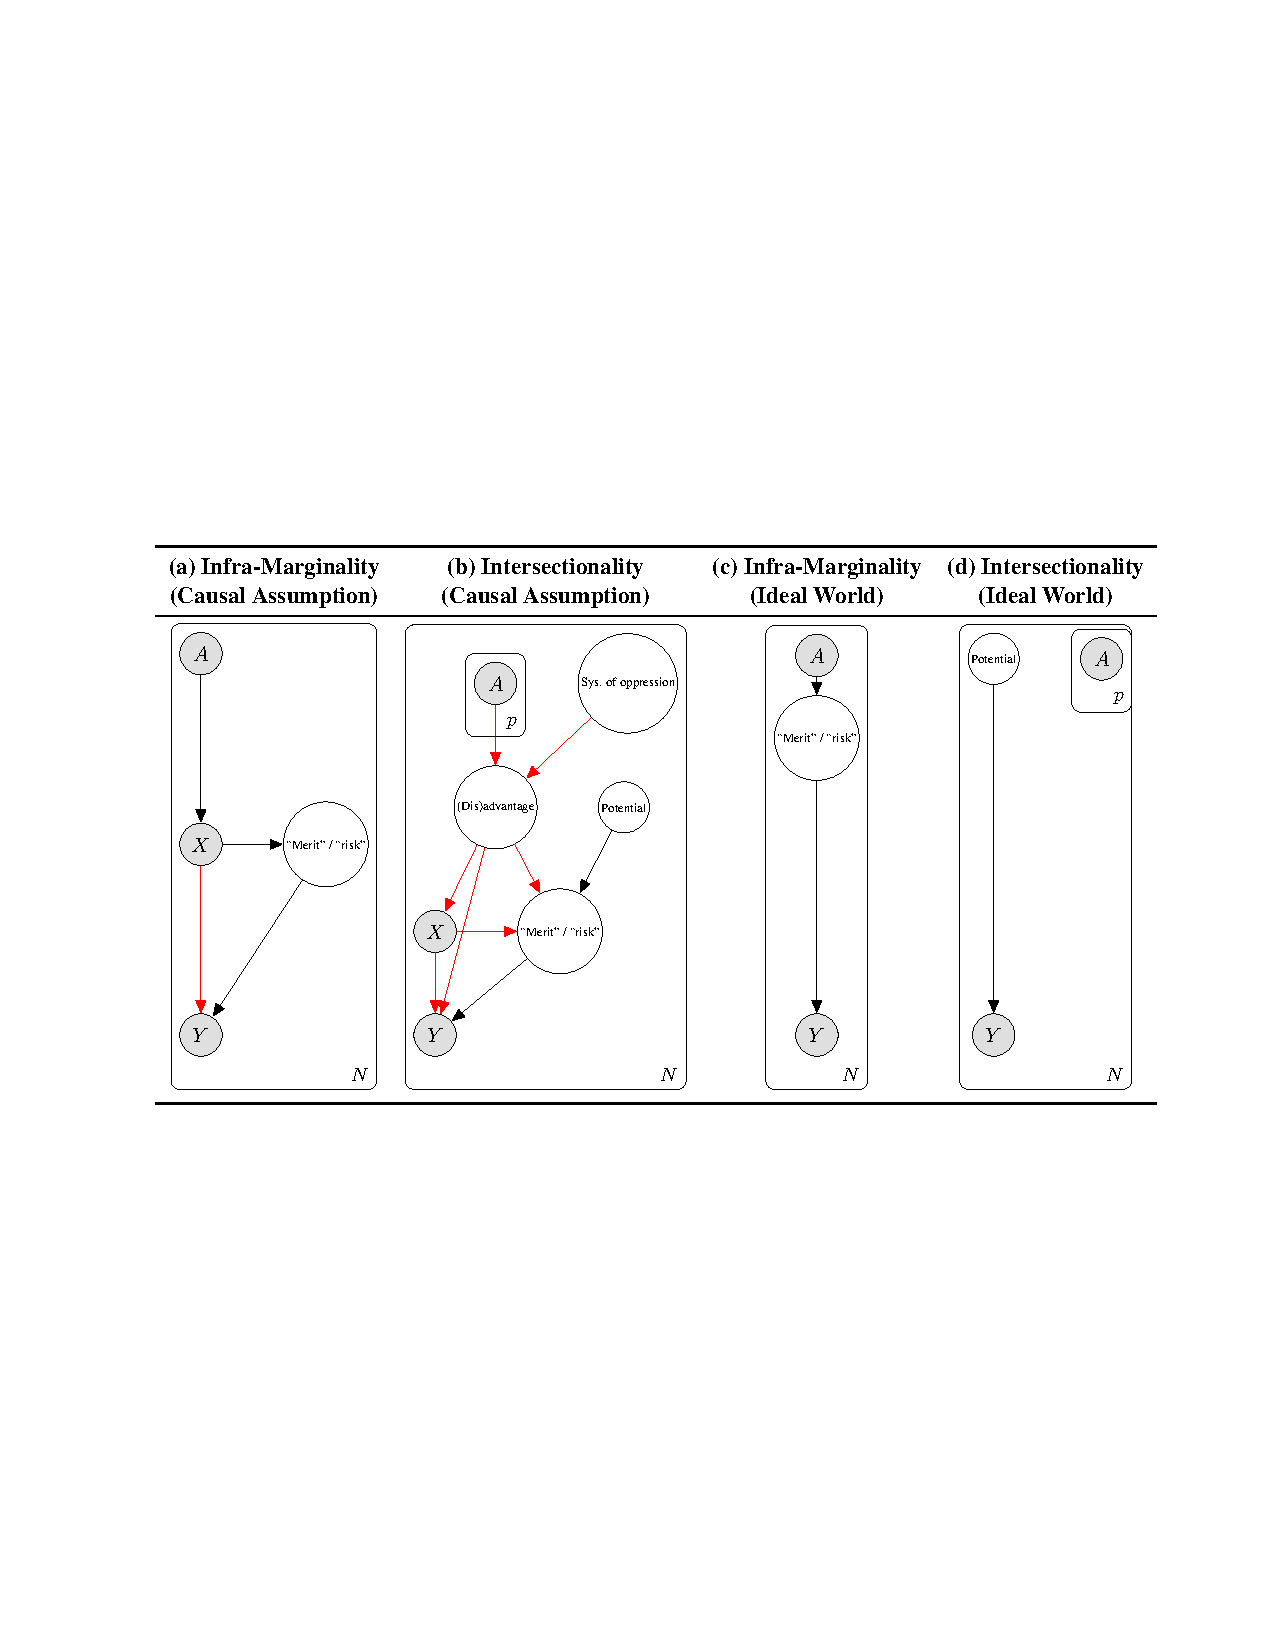
\includegraphics{figs/causalAssumptions}
	
%The following code generates the figures but isn't compatible with the \documentclass line		
%\begin{tabular}{cccc}
%	\toprule
%	\textbf{(a) Infra-Marginality} & \textbf{(b) Intersectionality} & \textbf{(c) Infra-Marginality} & \textbf{(d) Intersectionality} \\
%	\textbf{(Causal Assumption)} & \textbf{(Causal Assumption)} & \textbf{(Ideal World)} &  \textbf{(Ideal World)} \\ 
%	\midrule
%	\begin{tikzpicture}[y=2.44cm]%[x=2cm,y=3cm]
%		\node[obs] (Y) {$Y$} ;
%		\node[obs, above=of Y] (X) {$X$} ;
%		\node[latent, right=of X] (M) {\tiny ``Merit'' / ``risk''};
%		\node[obs, above=of X] (A) {$A$} ;
%		
%		\edge {A} {X}
%		\edge {X} {M}
%		\edge[red] {X} {Y}
%		\edge {M} {Y}
%		
%		\plate {infraPeople} {(A)(X)(M)(Y)} {$N$}
%	\end{tikzpicture}
%	 &
%	 
%	 \begin{tikzpicture}%[x=2cm,y=1.5cm]	 
%		 \node[obs] (Y) {$Y$} ;
%		 \node[obs, above=of Y] (X) {$X$} ;
%		 \node[latent, right=of X] (M) {\tiny ``Merit'' / ``risk''} ;
%		 \node[latent, above=of X, xshift = 1cm] (P) {\tiny (Dis)advantage} ;
%		 \node[latent, right=of P] (U) {\tiny Potential} ;
%		 \node[obs, above=of P] (A) {$A$} ;
%		 \node[latent, right=of A] (S) {\tiny Sys. of oppression} ;
%		 
%		 
%		 \edge[red] {A,S} {P}
%		 \edge[red] {P} {M}
%		 \edge[] {U} {M}
%		 \edge[red] {P} {X}
%		 \edge[red] {X} {M}
%		 \edge[red] {X} {Y}
%		 \edge {M} {Y}
%		 \edge[red] {P} {Y}
%		 
%		 \plate {interPeople} {(A)(X)(M)(Y)(P)(U)(S)} {$N$}
%		 \plate {interAtts} {(A)} {$p$}
%	 \end{tikzpicture}
%	&
%	\begin{tikzpicture}[y=3.85cm]%[x=2cm,y=3cm]
%		\node[obs] (Y) {$Y$} ;
%		\node[latent, above=of Y] (M) {\tiny ``Merit'' / ``risk''};
%		\node[obs, above=of X] (A) {$A$} ;
%		
%		\edge {A} {M}
%		\edge {M} {Y}
%		
%		\plate {infraIdealPeople} {(A)(M)(Y)} {$N$}	
%	\end{tikzpicture}
%	& 
%	\begin{tikzpicture}[y=5.44cm]%[x=2cm,y=2cm]	 
%	\node[obs] (Y) {$Y$} ;
%	\node[latent, above=of Y] (U) {\tiny Potential} ;
%	\node[obs, right=of U] (A) {$A$} ;	
%	
%	\edge {U} {Y}
%	
%	\plate {interPeople} {(A)(Y)(U)} {$N$}
%	\plate {interAtts} {(A)} {$p$}
%	\end{tikzpicture} \\
%	\bottomrule
%\end{tabular}
}
\caption{Implicit causal assumptions (a,b) and values-driven ideal world scenarios (c,d) for infra-marginality based \cite{corbettdavies2018measure,simoiu2017problem} and intersectionality-based \cite{crenshaw1989demarginalizing, collins2002black} perspectives on fairness \cite{foulds2020intersectional}. Here, $A$ denotes protected attributes, $X$ observed attributes, $Y$ outcomes, $N$ individuals, $p$ number of protected attributes.  Red arrows denote potentially unfair causal pathways, which are removed to obtain the ideal world scenarios (c,d). The above summarizes broad strands of research; individual works may differ. Note that in the intersectionality ideal world, protected attributes are $d$-separated from outcomes, which would imply that parity should occur, while this is not the case in the infra-marginality based ideal world which is willing to accept disparity. \label{fig:causalAssump}}
\end{figure*}


Also note that the inframarginality criticism is only relevant in scenarios where risk scores (or merit / qualifications) are used to assign favorable or unfavorable outcomes.  It does not pertain to other scenarios like recommendation, e.g. AI-based career counseling, where the class labels are not intrinsically better or worse than each other but we would still like to achieve parity \cite{Zeng,islam2020neural}. Lastly, race is a social construct and is not a well-defined biological property \cite{wagner2017anthropologists}.  Similarly, gender (as opposed to biological sex) is also a social construct \cite{west1987doing}.  Although racial and gender groups have diverse sets of lived experiences, there is little scientific evidence that there are legitimate biological differences in the ability levels of these groups \cite{wagner2017anthropologists, ellemers2018gender}.  Insinuations of such differences without clear supporting evidence can potentially veer into the realms of prejudice or scientific racism.

Regarding disparities due to confounders, as in the UC Berkeley graduate admissions case \cite{bickel1975sex}, this is a legitimate concern.  If known confounders exist, fairness methods which account for them should be used instead of simple parity-based methods, e.g. \cite{kusner2017counterfactual,nabi2018fair,nabi2019learning}.  Without complex causal modeling, a simple parity-based approach is to calculate parity-based fairness metrics conditioned on the confounder, as in the \emph{differential fairness with confounders} ($\epsilon$-DFC) metric proposed by the authors \cite{foulds2020intersectional}.  If confounders are unknown, it is difficult to prevent their impact on fairness measures, even ones based on causality, which typically require a causal model to be defined by the analyst.  In this case, we will argue below that the burden of proof for latent confounders may not lie with the organization which is developing the AI system in question.   
%\shimei{Please clarify "organization"} \jf{done} 
Yet, if researchers can identify confounders that impact parity post-deployment, they would be right to ask for the parity-based intervention to be modified or overturned.  Note also that \emph{systemic bias is itself a confounding variable} (cf. Figure \ref{fig:causalAssump} (b)).  If a causal model does not account for it in assessing fair outcomes, its inferences will not be fair or correct, either.  

\subsubsection{Response: Parity does not Prevent Certain Harms or Abuses, or Provide Certain Benefits} 
\label{sec:responseAbuses}

Recall that subset targeting, or fairness gerrymandering, is the issue that parity-based fairness methods do not protect against deliberate (or accidental) bias toward subgroups of the protected groups \cite{dwork2012fairness, kearns2018preventing}.  For example, if we enforce parity for gender and race, groups at the intersection of gender and race such as Black women are not necessarily protected, which is concerning from the perspective of intersectionality \cite{crenshaw1989demarginalizing}.  This problem can be mitigated by simply defining more fine-grained protected groups, e.g. designating Black women as protected.  Sophisticated parity-based fairness metrics have been proposed which automatically enforce parity for groups at the intersection of the protected attributes, including \emph{differential fairness (DF)} \cite{foulds2020intersectional} and \emph{statistical parity (SP) subgroup fairness} \cite{kearns2018preventing}.

Critics of the relationship between parity-based fairness and politically left-wing approaches such as affirmative action, particularly those who are concerned that they will be left behind by these ideas, are recommended to read the book ``\emph{Feminism is for Everybody}'' \cite{hooks2000feminism}.  The authors studied the related concern that \emph{some disadvantaged groups might be harmed by the fairness intervention} \cite{foulds2020intersectional}.  When enforcing our parity-based \emph{differential fairness} metric, which protects intersecting subgroups of protected groups, we found empirically that per-group fairness metrics were improved for almost every subgroup under consideration. 

Some of the other concerns we considered were that parity-based fairness could be achieved by badly behaved classifiers, such as those that deliberately select unqualified individuals to achieve parity, or by increasing negative outcomes.  One response to these types of concerns can be summarized by an old joke:
\begin{quote}
\emph{
``The patient says, `Doctor, it hurts when I do this.' \\
The doctor says, `Then don't do that!' ''} -- Henny Youngman, comedian.\footnote{\url{https://www.goodreads.com/author/quotes/82949.Henny_Youngman}}
\end{quote}
In other words, if these models are considered harmful, we can choose not to create them.    It is not reasonable to expect a single fairness definition to detect and prevent all possible bad behavior.  On the other hand, a healthy process for constructing fair AI should involve an engaged data scientist, plus ideally representatives of stakeholders, who should verify whether the behavior of the model is acceptable or pathological, beyond simply looking at chosen fairness metrics.  Once detected by an analyst, additional problems can be prevented by adding further penalties and constraints to the AI model, in addition to enforcing the parity-based metric.  Note that the \emph{self-fulfilling prophecy} issue (using the consequences of deliberate non-meritocratic parity to justify prejudice) was raised by privacy and security researchers \cite{dwork2012fairness}, whose field has a natural skepticism on human behavior.  While the skepticism may sometimes hold true, we anticipate that the vast majority fairness interventions will be made in good faith. 

Regarding benefits that parity-based fairness metrics do not achieve, such as individual guarantees, these are good reasons to consider using an alternative fairness metric.  They are not, however, reasons to dismiss parity-based fairness metrics out-of-hand as a useful tool for combating bias and fairness issues. For individual guarantees specifically, we would like to point out that parity-based fairness does confer a useful \emph{probabilistic} benefit to the individual: given their protected group, the prior probability of receiving a favorable outcome (before observing any attributes) will be similar to that of an individual from another group.  In the parity-based differential fairness metric \cite{foulds2020intersectional}, this translates to a privacy guarantee \emph{for individuals}: if an adversary sees your outcome $M(x)$, they will not be able to learn much about your protected attribute $s$.  

\subsection{Who has the Burden of Proof on Determining Whether Disparities are Legitimate?}

As we have discussed in Section \ref{sec:responseMeritocracy}, whether parity-based fairness interventions improve or degrade  the extent to which the classifier is meritocratic hinges on whether disparities in the data, which are replicated by the algorithm, are primarily due to unfair bias (from systemic bias, biased data annotation, etc), or are due to legitimate reasons (infra-marginality, confounders, etc).  Since bias is a complicated issue, it is rarely easy to answer this question.  When an organization decides whether or not to implement a parity-based fairness intervention, do they have the burden of proof on showing whether disparities are unfair?  In the absence of solid evidence, which assumption should be the default?

From a legal perspective, in the context of employment decisions in the United States protected by Title VII, if a plaintiff can demonstrate disparate impact (i.e. disparities in outcomes determined by a policy or algorithm), the burden of proof falls on the organization to demonstrate that the disparate impact is justified.  In other words, the organization must justify disparity due to its actions, but it need not justify parity due to its actions.  Thus, from a legal perspective, if the cause of the disparity is unknown it may be safest to assume that the disparity is unfair and apply a parity-based fairness intervention.\footnote{The authors of this paper are not legal experts and the statements in this paper should not be construed as legal advice.}

We may arrive at a similar conclusion from an ethical perspective.  If we incorrectly assume that a disparity is unjust and wrongly remove it, the harm falls on advantaged groups, and diversity/equity (a property which generally has intrinsic value) would be improved.  If we incorrectly assume that a disparity is just and wrongly choose not to address it, the harm falls on disadvantaged groups, and diversity/equity would not be improved.  The advantaged groups  typically have more resources than the disadvantaged groups and are in a better position to shoulder the burden, so the overall impact is less if those groups are harmed.  If we make a wrong choice, meritocracy is harmed either way to the same degree (the size of the intervention).  Therefore, supposing there is a 50/50 or greater chance that the disparity is unjust, the least amount of expected harm occurs if we choose to perform a parity-based fairness intervention.  All other things being equal, in a situation where we have good reason to suspect that a disparity of outcomes is unjust ---such as scientific studies showing discrimination in similar settings--- and we have no reason to suspect that the disparity of outcomes is legitimate ---e.g. one demographic is legitimately more qualified than another or there are known confounders---, performing a parity-based fairness intervention may be a better choice than doing nothing at all, supposing that we do so in a manner that does not substantially harm system performance.  Of course, if there is another fairness intervention that is more appropriate in our particular context, we should consider performing that intervention instead.

\subsection{Summary of our Findings}

Based on the analysis in this paper, we have yet to see a compelling argument that parity-based fairness metrics are invalid in all contexts.  We do not agree with \cite{Hardt2016approaching} that parity-based fairness metrics are ``fundamentally flawed.'' Parity-based fairness advances the intrinsically valuable ideal of equality, can rectify societal bias, can prevent bias from unfair class labels, and has economic and legal benefits in some contexts.  We have also seen that parity-based fairness is not always ideal, and there are a number of useful arguments regarding the limitations of parity-based fairness in some contexts and under some value systems.  The existence of limitations does not however completely preclude its use.  Some of these limitations can be partially mitigated within a parity-based approach, while in other cases may be best addressed by the use of alternative fairness metrics such as equalized odds, individual fairness, or causal fairness definitions.  These alternative fairness metrics have their own limitations, and none can conclusively be argued to be superior to parity-based fairness in all contexts.

% -Must a fairness definition prevent all possible evils to be considered valid, including ones that can be prevented by design or otherwise checked?
%   -Is the goal to achieve (perfect) fairness, or to reduce bias/discrimination?  If we are doing fairness, maybe our metric has to capture what it philosophically means to be fair.  But this seems impossible, especially since fairness is highly contested for centuries, and is highly context dependent.  If we are doing bias reduction, it doesn't matter if our metric is a perfect barometer for justice, as long as it leads to a beneficial intervention. 

% -It isn't fair to dismiss a fairness intervention due to its behavior in the most extreme settings, when more moderate settings can be chosen.

% -In some cases, other metrics are preferable.  That does not mean that parity-based fairness is not a useful construct.

% -``A fairness definition has limitations and does not apply in all contexts'' is not a reason to dismiss it out of hand.  Every fairness definition has limitations, including the competing definitions to parity-based metrics.  If you can imagine a scenario where it is inappropriate, don't use it in that scenario. 

% -For detractors to argue that a fairness metric is too flawed to be used, they must show that it causes more harm than good (or less benefit than alternatives) in all contexts.  They have not done so. 

%Case study: university admissions?

\section{Guidelines and Recommendations}

Informed by the above discussion we now provide a set of guidelines and recommendations to the community regarding parity-based fairness metrics.

\subsection{Guidelines on Using Parity-Based Fairness Interventions}

The technique of penalizing or constraining a machine learning algorithm to enforce a parity-based fairness metric is useful in many contexts, but it must be used with care.  Due to its various limitations, it is not appropriate in all contexts.  We must carefully consider the relevant properties of the AI task at hand and its broader socio-technical context before determining whether to proceed.  We propose the following set of guidelines to be used as a ``pre-flight checklist'' on whether and how to use a parity-based fairness intervention.  This list is only a guideline, not a prescription, and it is almost certainly not complete. It is important to further consider the nuances of the particular application.  Several of these guidelines apply more broadly to all of fair AI. 
 
\begin{enumerate}

 \item When developing an AI fairness intervention, including the choice of fairness metric to uphold in a fair learning algorithm, it is important to consider contextual factors such as who is harmed, what is the nature of the harm, how does it relate to historical injustices, and stakeholder involvement in the design of the fair AI system, particularly stakeholders who are underrepresented within the organization \cite{crawford2019ai}.
 
 \item Before using any fairness intervention or deploying a fairness-sensitive system without one, practitioners should make a best-effort attempt to understand whether disparities of class labels in the data are substantially due to unfair reasons or to legitimate reasons.  If this cannot be determined from available data, scientific studies on related settings may suggest whether unfair bias is likely in the current context.
 
 \item If the disparity is due to legitimate reasons, e.g. there are known legitimate differences in ability between groups (infra-marginality), parity-based fairness metrics are not appropriate.  Consider using threshold tests instead. 

 \item If there are known confounders, parity-based fairness metrics are not appropriate.  Parity-based metrics which account for confounders such as $\epsilon$-DFC, or causal methods, should be used instead.
 
 \item If strong individual-level guarantees are essential for the application, individual fairness should be used instead.  Similarly, if there are other essential fairness properties that are only ensured by a different definition, that definition should be used instead. 

 \item If harm by the system is due to making prediction errors rather than from not receiving a favorable outcome, equalized odds or equality of opportunity are more appropriate fairness definitions.
 
 \item If it is suspected that disparities of class labels are substantially unfair (e.g. due to societal bias or annotation bias), disparities cause a harm of representation, or equality is important for the application regardless of unfairness in the data, parity-based fairness metrics are a good candidate to be used.
 
 \item If there is uncertainty over whether disparities of class labels are unfair, but there is reasonable suspicion that this is the case and there is no evidence of infra-marginality or confounding, it may be better to perform a parity-based fairness intervention than to make no fairness intervention.  Wrongly making a parity-based fairness intervention may be less harmful than wrongly failing to make a parity-based fairness intervention.  This assumes that the intervention is done such that little reduction in accuracy occurs, and that there is not another more appropriate fairness intervention for this context. 
 
 \item If it is important to maintain a high level of classification accuracy for this application, choose appropriate fairness hyper-parameter settings to achieve this.  We generally recommend using a grid search on a validation set to select fairness hyper-parameters, such that fairness is the best achievable under the constraint that accuracy decrease (or another performance metric) is within (say) 95\% of the performance of the typical model (accuracy $\times \ 0.95$).
 
 \item If no loss in accuracy at all is acceptable, consider setting a threshold on the fairness penalty such that only an increase in disparity over the existing disparity in the data is penalized.  This strategy only prevents ``bias amplification'' due to the algorithm's behavior, e.g. from overfitting.
 
 \item If we have strong evidence that most of the disparity is due to unfair reasons, a strict parity-based fairness constraint may be appropriate, even at a substantial cost to accuracy, since an accurate classifier cannot be a fair one in that case.
  
 \item After deployment, it is important to continue to monitor the fairness of the system and to continue to learn about the nature of the unfairness in the data and the system, and adapt the intervention accordingly.  For example, if external researchers or activists identify a flaw in the fairness of the system, corresponding adjustments should be made. 


\end{enumerate}
  
\subsection{Recommendations to the Community}

After considering the many arguments on both sides of the issue, we conclude that parity-based fairness metrics remain a valid and desirable notion of fair AI behavior in many 
%\shimei{How about replacing "some" with "many"?}\jf{done}
contexts.  We therefore \textbf{call upon community members 
%\shimei{how about replacing "peer reviewers" with "community members" since  not just "peer reviewers" need to pay attention to this }\jf{done.  I instead mentioned peer review as important in the next sentence, though. I emphasize it because I want this paper to be a reference for authors to use in their rebuttals if they encounter these criticisms during peer review}
to cease the practice of dismissing fundamental methods-oriented AI fairness research on parity-based fairness metrics out-of-hand}, due to perceived limitations of the approach. \emph{This is particularly important during peer review}.  It is however appropriate to critique \emph{applied AI fairness research} 
%\shimei{How about removing "during peer review". Although it is important in terms of publication, most people care more about the real impact of deployed systems than publications. }\jf{done}
regarding the limitations of any chosen fairness metric (parity-based or otherwise) relative to alternatives \emph{in the context of a particular application}, as long as political impartiality is maintained as much as possible.  For example, debate and critiques regarding the appropriate metrics to evaluate the fairness of the COMPAS criminal recidivism predictor \cite{angwin2016machine} are valuable and would have been appropriate in peer review of a paper describing the COMPAS system.  We request that peer reviewers endeavor to prevent their own political views and value systems from impacting their assessment of AI fairness research.

We further suggest that the debate around parity-based fairness  should remain civil in highly public settings such as in audience questions after conference talks and on social media.  In those contexts there are often impassioned, sometimes even angrily stated objections to parity-based fairness, as the authors of this paper have witnessed first-hand.  The presently ongoing debate around the firing of Timnit Gebru by Google is emblematic of the high tensions in this area.  While debate around these issues must continue and we do not intend to stifle it, unjustified vitriolic attacks on parity-based fairness research can have a chilling effect on a much-needed area of study, and they do nothing to advance the discussion. 
%\shimei{Again, conference Q\&A sessions or even social media can be an appropriate venue for this type of discussion/debate/criticism as long as people remain civil. Otherwise, where should the debate/discussion occur? Suggest to remove the part in the above paragraph that sounds personal.} \jf{I modified to simply request civility.  I have left in the personal part but I rearranged the sentence to reduce the importance of the personal dimension.  It is there to support the claim - we have seen first hand that this happens, so we don't need to cite other evidence for it.}
%\shimei{Thank you for the revision. I like the current version much better.}
%JF: ok, commenting this out since it seems to be addressed.


% \begin{figure}
% 	\centering
% 	
\includegraphics{figs/myfigure.png}
	
% 	\caption{An example figure.}
	
% \end{figure}
 

\section{Conclusions}
Despite their widespread use, parity-based AI fairness metrics have been somewhat controversial in some circles due to various limitations that have been put forward in the literature.  We discussed the pros and cons of these metrics when used as a penalty or constraint to enforce AI fairness in a machine learning system.  In many contexts, parity-based fairness confers useful benefits such as mitigating unfair disparities, improving diversity, and reducing legal liability.  Although many important concerns have been raised such as potentially reducing prediction accuracy or unfair impacts when they are used to remove legitimate disparities, mitigation strategies exist, and none of the concerns would preclude the use of the methodology in all contexts.  We conclude that although parity-based fairness metrics are not a panacea, and there are situations where they are not appropriate or other fairness metrics would be preferable, they remain useful tools in the AI fairness practitioner's toolkit.

\section{Acknowledgments}
We thank Rosie Kar for valuable insights regarding intersectionality and standpoint theory. This work was performed under the following financial assistance award: 60NANB18D227 from U.S. Department of Commerce, National Institute of Standards and Technology. This material is based upon work supported by the National Science Foundation under Grant Nos IIS 1850023; IIS1927486.  Any opinions, findings, and conclusions or recommendations expressed in this material are those of the author(s) and do not necessarily reflect the views of the National Science Foundation.

\newpage
 
\vspace{-.1cm}
%\bibliographystyle{ACM-Reference-Format}
%\bibliographystyle{apalike}
%\bibliography{references}

\begin{thebibliography}{}
	
	\bibitem[Alexander, 2012]{alexander2012new}
	Alexander, M. (2012).
	\newblock {\em The new Jim Crow: Mass incarceration in the age of
		colorblindness}.
	\newblock T. N. P.
	
	\bibitem[Angwin et~al., 2016]{angwin2016machine}
	Angwin, J., Larson, J., Mattu, S., and Kirchner, L. (2016).
	\newblock Machine bias: There's software used across the country to predict
	future criminals. and it's biased against blacks.
	\newblock {\em ProPublica, May}, 23.
	
	\bibitem[Ayres, 2002]{ayres2002outcome}
	Ayres, I. (2002).
	\newblock Outcome tests of racial disparities in police practices.
	\newblock {\em Justice research and Policy}, 4(1-2):131--142.
	
	\bibitem[Barocas and Selbst, 2016]{barocas2016big}
	Barocas, S. and Selbst, A. (2016).
	\newblock Big data's disparate impact.
	\newblock {\em Cal. L. Rev.}, 104:671.
	
	\bibitem[Barrett et~al., 2019]{barrett2019emotional}
	Barrett, L.~F., Adolphs, R., Marsella, S., Martinez, A.~M., and Pollak, S.~D.
	(2019).
	\newblock Emotional expressions reconsidered: Challenges to inferring emotion
	from human facial movements.
	\newblock {\em Psychological science in the public interest}, 20(1):1--68.
	
	\bibitem[Beede et~al., 2011]{beede2011women}
	Beede, D.~N., Julian, T.~A., Langdon, D., McKittrick, G., Khan, B., and Doms,
	M.~E. (2011).
	\newblock Women in stem: A gender gap to innovation.
	\newblock {\em Economics and Statistics Administration Issue Brief}, 04-11.
	
	\bibitem[Bell et~al., 2011]{bell2011voice}
	Bell, M.~P., {\"O}zbilgin, M.~F., Beauregard, T.~A., and S{\"u}rgevil, O.
	(2011).
	\newblock Voice, silence, and diversity in 21st century organizations:
	Strategies for inclusion of gay, lesbian, bisexual, and transgender
	employees.
	\newblock {\em Human resource management}, 50(1):131--146.
	
	\bibitem[Berk et~al., 2018]{berk2017fairness}
	Berk, R., Heidari, H., Jabbari, S., Kearns, M., and Roth, A. (2018).
	\newblock Fairness in criminal justice risk assessments: The state of the art.
	\newblock {\em In Sociological Methods and Research}, 1050:28.
	
	\bibitem[Bickel et~al., 1975]{bickel1975sex}
	Bickel, P.~J., Hammel, E.~A., and O'Connell, J.~W. (1975).
	\newblock Sex bias in graduate admissions: Data from {B}erkeley.
	\newblock {\em Science}, 187(4175):398--404.
	
	\bibitem[Buolamwini and Gebru, 2018]{buolamwini2018gender}
	Buolamwini, J. and Gebru, T. (2018).
	\newblock Gender shades: Intersectional accuracy disparities in commercial
	gender classification.
	\newblock In {\em FAT*}.
	
	\bibitem[Collins, 1990]{collins2002black}
	Collins, P. (2002 [1990]).
	\newblock {\em Black feminist thought: Knowledge, consciousness, and the
		politics of empowerment (2nd ed.)}.
	\newblock Routledge.
	
	\bibitem[{Combahee River Collective}, 1978]{collective1977black}
	{Combahee River Collective} (1978).
	\newblock A {B}lack feminist statement.
	\newblock In Eisenstein, Z., editor, {\em Capitalist Patriarchy and the Case
		for Socialist Feminism}. Monthly Review Press, New York.
	
	\bibitem[Corbett-Davies and Goel, 2018]{corbettdavies2018measure}
	Corbett-Davies, S. and Goel, S. (2018).
	\newblock The measure and mismeasure of fairness: A critical review of fair
	machine learning.
	
	\bibitem[Cox and Blake, 1991]{cox1991managing}
	Cox, T.~H. and Blake, S. (1991).
	\newblock Managing cultural diversity: Implications for organizational
	competitiveness.
	\newblock {\em Academy of Management Perspectives}, 5(3):45--56.
	
	\bibitem[Crawford et~al., 2019]{crawford2019ai}
	Crawford, K., Dobbe, R., Dryer, T., Fried, G., Green, B., Kaziunas, E., Kak,
	A., Mathur, V., McElroy, E., S{\'a}nchez, A.~N., et~al. (2019).
	\newblock {AI} {N}ow 2019 report.
	\newblock {\em New York, NY: AI Now Institute}.
	
	\bibitem[Crenshaw, 1989]{crenshaw1989demarginalizing}
	Crenshaw, K. (1989).
	\newblock Demarginalizing the intersection of race and sex: A {B}lack feminist
	critique of antidiscrimination doctrine, feminist theory and antiracist
	politics.
	\newblock {\em U. Chi. Legal F.}, pages 139--167.
	
	\bibitem[Dastin, 2018]{dastin2018amazon}
	Dastin, J. (2018).
	\newblock Amazon scraps secret {AI} recruiting tool that showed bias against
	women.
	\newblock {\em Reuters}.
	
	\bibitem[Davis, 2011]{davis2011prisons}
	Davis, A. (2011).
	\newblock {\em Are prisons obsolete?}
	\newblock Seven Stories Press.
	
	\bibitem[Deshpande et~al., 2020]{ketki}
	Deshpande, K.~V., Pan, S., and Foulds, J.~R. (2020).
	\newblock Mitigating demographic bias in {AI}-based resume filtering.
	\newblock In {\em UMAP '20 Adjunct}, page 268–275. Association for Computing
	Machinery.
	
	\bibitem[Dionne, 2004]{dionne2004americans}
	Dionne, E.~J. (2004).
	\newblock {\em Why Americans hate politics}.
	\newblock Simon and Schuster.
	
	\bibitem[Dwork et~al., 2012]{dwork2012fairness}
	Dwork, C., Hardt, M., Pitassi, T., Reingold, O., and Zemel, R. (2012).
	\newblock Fairness through awareness.
	\newblock In {\em Proceedings of ITCS}, pages 214--226.
	
	\bibitem[Ellemers, 2018]{ellemers2018gender}
	Ellemers, N. (2018).
	\newblock Gender stereotypes.
	\newblock {\em Annual review of psychology}, 69:275--298.
	
	\bibitem[{Equal Employment Opportunity Commission}, 1978]{eeoc1966guidelines}
	{Equal Employment Opportunity Commission} (1978).
	\newblock Guidelines on employee selection procedures.
	\newblock {\em C.F.R.}, 29.1607.
	
	\bibitem[Foulds et~al., 2020]{foulds2020bayesian}
	Foulds, J.~R., Islam, R., Keya, K.~N., and Pan, S. (2020).
	\newblock Bayesian modeling of intersectional fairness: The variance of bias.
	\newblock In {\em Proceedings of the 2020 SIAM International Conference on Data
		Mining}, pages 424--432. SIAM.
	
	\bibitem[{Foulds} et~al., 2020]{foulds2020intersectional}
	{Foulds}, J.~R., {Islam}, R., {Keya}, K.~N., and {Pan}, S. (2020).
	\newblock An intersectional definition of fairness.
	\newblock In {\em 2020 IEEE 36th International Conference on Data Engineering
		(ICDE)}, pages 1918--1921.
	
	\bibitem[Grant et~al., 2011]{grant2011injustice}
	Grant, J., Mottet, L., Tanis, J., Harrison, J., Herman, J., and Keisling, M.
	(2011).
	\newblock {\em Injustice at every turn: A report of the national transgender
		discrimination survey}.
	\newblock National Center for Transgender Equality.
	
	\bibitem[Hardt, 2016]{Hardt2016approaching}
	Hardt, M. (2016).
	\newblock Approaching fairness in machine learning.
	\newblock [Online; posted September 6, 2016]
	\url{http://blog.mrtz.org/2016/09/06/approaching-fairness.html}.
	
	\bibitem[Hardt et~al., 2016]{hardt2016equality}
	Hardt, M., Price, E., Srebro, N., et~al. (2016).
	\newblock Equality of opportunity in supervised learning.
	\newblock In {\em Advances in NeurIPS}, pages 3315--3323.
	
	\bibitem[Hartsock, 1983]{hartsock1983feminist}
	Hartsock, N.~C. (1983).
	\newblock The feminist standpoint: Developing the ground for a specifically
	feminist historical materialism.
	\newblock In {\em Discovering reality}, pages 283--310. Springer.
	
	\bibitem[hooks, 1981]{hooks1981ain}
	hooks, b. (1981).
	\newblock {\em Ain't {I} a Woman: Black Women and Feminism}.
	\newblock South End Press.
	
	\bibitem[hooks, 2000]{hooks2000feminism}
	hooks, b. (2000).
	\newblock {\em Feminism is for everybody: Passionate politics}.
	\newblock Pluto Press.
	
	\bibitem[Islam et~al., 2020]{islam2020neural}
	Islam, R., Keya, K.~N., Zeng, Z., Pan, S., and Foulds, J. (2020).
	\newblock Neural fair collaborative filtering.
	
	\bibitem[Jefferson, 2018]{constitution}
	Jefferson, T. (2018).
	\newblock {\em The Papers of Thomas Jefferson, Volume 21: Index}, volume~1.
	\newblock Princeton University Press.
	
	\bibitem[Johnson, 1965]{johnson1965remarks}
	Johnson, L.~B. (1965).
	\newblock {\em Commencement Address at Howard University: ``To Fulfill These
		Rights''}.
	\newblock Howard University.
	
	\bibitem[Kearns et~al., 2018]{kearns2018preventing}
	Kearns, M., Neel, S., Roth, A., and Wu, Z. (2018).
	\newblock Preventing fairness gerrymandering: Auditing and learning for
	subgroup fairness.
	\newblock In {\em Proc. of ICML, PMLR 80}, pages 2569--2577.
	
	\bibitem[Kearns et~al., 2019]{kearns2019average}
	Kearns, M., Roth, A., and Sharifi-Malvajerdi, S. (2019).
	\newblock Average individual fairness: Algorithms, generalization and
	experiments.
	\newblock In {\em Advances in Neural Information Processing Systems}, pages
	8242--8251.
	
	\bibitem[Keya et~al., 2020]{keya2020equitable}
	Keya, K.~N., Islam, R., Pan, S., Stockwell, I., and Foulds, J.~R. (2020).
	\newblock Equitable allocation of healthcare resources with fair {C}ox models.
	
	\bibitem[Keyes et~al., 2019]{keyes2019mulching}
	Keyes, O., Hutson, J., and Durbin, M. (2019).
	\newblock A mulching proposal: Analysing and improving an algorithmic system
	for turning the elderly into high-nutrient slurry.
	\newblock In {\em Extended Abstracts of the 2019 CHI Conference on Human
		Factors in Computing Systems}. ACM.
	
	\bibitem[Kusner et~al., 2017]{kusner2017counterfactual}
	Kusner, M., Loftus, J., Russell, C., and Silva, R. (2017).
	\newblock Counterfactual fairness.
	\newblock In {\em NeurIPS}.
	
	\bibitem[Landeau, 2020]{Landeau2020}
	Landeau, A. (2020).
	\newblock Measuring fairness in machine learning models.
	\newblock [Online; posted September 18-2020].
	
	\bibitem[Lorde, 1984]{lorde1984age}
	Lorde, A. (1984).
	\newblock Age, race, class, and sex: Women redefining difference.
	\newblock In {\em Sister Outsider}, pages 114--124. Ten Speed Press.
	
	\bibitem[Lowry and Macpherson, 1988]{lowry1988blot}
	Lowry, S. and Macpherson, G. (1988).
	\newblock A blot on the profession.
	\newblock {\em British medical journal (Clinical research ed.)}, 296(6623):657.
	
	\bibitem[Nabi et~al., 2019]{nabi2019learning}
	Nabi, R., Malinsky, D., and Shpitser, I. (2019).
	\newblock Learning optimal fair policies.
	\newblock {\em Proceedings of machine learning research}, 97:4674.
	
	\bibitem[Nabi and Shpitser, 2018]{nabi2018fair}
	Nabi, R. and Shpitser, I. (2018).
	\newblock Fair inference on outcomes.
	\newblock In {\em Proceedings of the AAAI Conference on Artificial
		Intelligence}, volume 2018, page 1931.
	
	\bibitem[Nedlund, 2019]{applecard}
	Nedlund, E. (2019).
	\newblock Apple card is accused of gender bias. here's how that can happen.
	\newblock [CNN Business. Online; posted November 12,2019]
	\url{https://www.cnn.com/2019/11/12/business/apple-card-gender-bias/index.html}.
	
	\bibitem[Noble, 2018]{noble2018algorithms}
	Noble, S. (2018).
	\newblock {\em Algorithms of Oppression: How Search Engines Reinforce Racism}.
	\newblock NYU Press.
	
	\bibitem[Page, 2008]{page2008difference}
	Page, S.~E. (2008).
	\newblock {\em The difference: How the power of diversity creates better
		groups, firms, schools, and societies-new edition}.
	\newblock Princeton University Press.
	
	\bibitem[Simoiu et~al., 2017]{simoiu2017problem}
	Simoiu, C., Corbett-Davies, S., Goel, S., et~al. (2017).
	\newblock The problem of infra-marginality in outcome tests for discrimination.
	\newblock {\em The Annals of Applied Statistics}, 11(3):1193--1216.
	
	\bibitem[Truth, 1851]{truth1851aint}
	Truth, S. (1851).
	\newblock Ain't {I} a woman?
	\newblock Speech delivered at Women's Rights Convention, Akron, Ohio.
	
	\bibitem[Vanian, 2019]{HateSpeechDetectionBias}
	Vanian, J. (2019).
	\newblock Google’s hate speech detection {A.I.} has a racial bias problem.
	\newblock [Fortune. Online; posted August 16, 2019]
	\url{https://fortune.com/2019/08/16/google-jigsaw-perspective-racial-bias/}.
	
	\bibitem[Verma and Rubin, 2018]{20plusdefinitionssuervey}
	Verma, S. and Rubin, J. (2018).
	\newblock Fairness definitions explained.
	\newblock In {\em Proceedings of the International Workshop on Software
		Fairness}, pages 1--7. Association for Computing Machinery.
	
	\bibitem[Verschelden, 2017]{verschelden2017bandwidth}
	Verschelden, C. (2017).
	\newblock {\em Bandwidth Recovery: Helping Students Reclaim Cognitive Resources
		Lost to Poverty, Racism, and Social Marginalization}.
	\newblock Stylus.
	
	\bibitem[Wagner et~al., 2017]{wagner2017anthropologists}
	Wagner, J.~K., Yu, J.-H., Ifekwunigwe, J.~O., Harrell, T.~M., Bamshad, M.~J.,
	and Royal, C.~D. (2017).
	\newblock Anthropologists' views on race, ancestry, and genetics.
	\newblock {\em American Journal of Physical Anthropology}, 162(2):318--327.
	
	\bibitem[Weisskopf, 2004]{weisskopf2004affirmative}
	Weisskopf, T.~E. (2004).
	\newblock {\em Affirmative action in the United States and India: A comparative
		perspective}.
	\newblock Routledge.
	
	\bibitem[West and Zimmerman, 1987]{west1987doing}
	West, C. and Zimmerman, D.~H. (1987).
	\newblock Doing gender.
	\newblock {\em Gender \& society}, 1(2):125--151.
	
	\bibitem[Zafar et~al., 2017a]{zafar2015fairness}
	Zafar, M., Valera, I., Rodriguez, M., and Gummadi, K. (2017a).
	\newblock Fairness constraints: Mechanisms for fair classification.
	\newblock In {\em AISTATS}.
	
	\bibitem[Zafar et~al., 2017b]{zafar2017parity}
	Zafar, M.~B., Valera, I., Rodriguez, M., Gummadi, K., and Weller, A. (2017b).
	\newblock From parity to preference-based notions of fairness in
	classification.
	\newblock In {\em Advances in Neural Information Processing Systems}, pages
	229--239.
	
	\bibitem[Zeng et~al., 2021]{Zeng}
	Zeng, Z., Islam, R., Keya, K., Foulds, J., Song, Y., and Pan., S. (2021).
	\newblock Fair heterogeneous network embeddings.
	\newblock In {\em Proceedings of the 15th International AAAI Conference on Web
		and Social Media (Accepted)}. AAAI.
	
	\bibitem[Zhao et~al., 2017]{zhao2017men}
	Zhao, J., Wang, T., Yatskar, M., Ordonez, V., and Chang, K.-W. (2017).
	\newblock Men also like shopping: Reducing gender bias amplification using
	corpus-level constraints.
	\newblock In {\em Proceedings of EMNLP}.
	
\end{thebibliography}



%%%%% Example bibliography using bibitems
% \begin{thebibliography}{10}
% \begin{small}
% \itemsep=-.5pt
% \bibitem{1}
% Athanassoulis, Manos ; Johnson, Ryan ; Ailamaki, Anastasia ; Stoica, Radu, Improving OLTP Concurrency through Early Lock Release, EPFL-REPORT-152158, https://infoscience.epfl.ch/record/152158?ln=en, 2009. 

% \bibitem{2}
% Azure CosmosDB, https://azure.microsoft.com/en-us/services/cosmos-db/ 

% \bibitem{3}
% Bernstein, P.A., M., T. Kiefer, D. Maier: Indexing in an Actor-Oriented Database. CIDR 2017  

% \bibitem{4}
% Bernstein, P. A., E. Newcomer: Chapter 10: Transactional Middleware Products and Standards, in Principles of Transaction Processing, Morgan Kaufmann, 2nd ed., 2009. 

% \bibitem{5}
% Chang, F., J. Dean, S. Ghemawat, W.C. Hsieh, D.A. Wallach, M. Burrows, T. Chandra, A. Fikes, R.E. Gruber: Bigtable: A Distributed Storage System for Structured Data. ACM Trans. Comput. Syst. 26(2): 4:1-4:26 (2008) 


% \bibitem{6}
% %Corbett, J.C., J. Dean, M. Epstein, A. Fikes, C. Frost, J.J. Furman, S. Ghemawat, A. Gubarev, C. Heiser, P. Hochschild, W.C. Hsieh, S. Kanthak, E. Kogan, H. Li, A. Lloyd, S. Melnik, D. Mwaura, D. Nagle, S. Quinlan, R. Rao, L. Rolig, Y. Saito, M. Szymaniak, C. Taylor, R. Wang, D. Woodford: Spanner: Google's Globally Distributed Database. ACM Trans. Comput. Syst. 31(3): 8:1-8:22 (2013) 
% Corbett, J.C. et al: Spanner: Google's Globally Distributed Database. ACM Trans. Comput. Syst. 31(3): 8:1-8:22 (2013) 
% \bibitem{7}
% DeWitt, D.J., R.H. Katz, F. Olken, L.D. Shapiro, M. Stonebraker, D.A. Wood: Implementation Techniques for Main Memory Database Systems. SIGMOD 1984: 1-8 

% \bibitem{8}
% DynamoDB, https://aws.amazon.com/dynamodb/ 

% \bibitem{9}
% Eldeeb, T. and P. Bernstein: Transactions for Distributed Actors in the Cloud. Microsoft Research Tech Report MSR-TR-2016-1001. 

% \bibitem{10}
% Graefe, G., M. Lillibridge, H. A. Kuno, J. Tucek, A.C. Veitch: Controlled lock violation. SIGMOD 2013: 85-96 

% \bibitem{11}
% Helland, P., Life beyond Distributed Transactions: an Apostate's Opinion. CIDR 2007: 132-141 

% \bibitem{12}
% Java EE documentation, http://www.oracle.com/technetwork/?java/javaee/documentation/index.html  

% \bibitem{13}
% Larson, P-A, et al.: High-Perf. Concurrency Control Mechanisms for Main-Memory Databases. PVLDB 2011 
% \bibitem{14}

% Levandoski, L.J., D.B. Lomet, S. Sengupta, R. Stutsman, R. Wang: High Performance Transactions in Deuteronomy. CIDR 2015 

% \bibitem{15}
% David B. Lomet: Using Timestamping to Optimize Two Phase Commit. PDIS 1993: 48-55 

% \bibitem{16}
% Orleans, http://dotnet.github.io/orleans 

% \bibitem{18}
% The Open Group, Distributed Transaction Processing: The XA Specification, http://pubs.opengroup.org/onlinepubs/009680699/toc.pdf. 

% \bibitem{19}
% Vogels W., Eventually Consistent. ACM Queue 6(6): 14-19 (2008) \end{small}
% \end{thebibliography}

\end{document}
